\documentclass[10pt]{beamer}

% Beamer style
%\usetheme[secheader]{Madrid}
\usetheme{CambridgeUS}
\usecolortheme[rgb={0.65,0.15,0.25}]{structure}
%\usefonttheme[onlymath]{serif}
\beamertemplatenavigationsymbolsempty
%\AtBeginSubsection

% Packages
%\usepackage[french]{babel}
\usepackage[latin1]{inputenc}
\usepackage{color}
\usepackage{dsfont, stmaryrd}
\usepackage{amsmath, amsfonts, amssymb}
\usepackage{stmaryrd}
\usepackage{epsfig}
\usepackage{/home/robin/LATEX/Biblio/astats}
%\usepackage[all]{xy}
\usepackage{graphicx}

% Commands
\definecolor{darkred}{rgb}{0.65,0.15,0.25}
\definecolor{darkgreen}{rgb}{0,0.4,0}
\newcommand{\emphase}[1]{\textcolor{darkred}{#1}}
%\newcommand{\emphase}[1]{\textcolor{black}{#1}}
\newcommand{\paragraph}[1]{\textcolor{darkred}{#1}}
\newcommand{\refer}[1]{\textcolor{blue}{[\cite{#1}]}}
\newcommand{\Refer}[1]{\textcolor{blue}{[#1]}}
\newcommand{\newblock}{}

% Symbols
\newcommand{\Beta}{\text{Beta}}
\newcommand{\Bcal}{\mathcal{B}}
\newcommand{\dd}{\text{d}}
\newcommand{\Esp}{\mathbb{E}}
\newcommand{\Kbf}{{\bf K}}
\newcommand{\Gcal}{\mathcal{G}}
\newcommand{\Gam}{\mathcal{G}\text{am}}
\newcommand{\Ibb}{\mathbb{I}}
\newcommand{\Var}{\mathbb{V}}
\newcommand{\Fcal}{\mathcal{F}}
\newcommand{\Hcal}{\mathcal{H}}
\newcommand{\Lcal}{\mathcal{L}}
\newcommand{\Mcal}{\mathcal{M}}
\newcommand{\mubf}{\text{\mathversion{bold}{$\mu$}}}
\newcommand{\Ncal}{\mathcal{N}}
\newcommand{\Nbf}{{\bf N}}
\newcommand{\Nm}{N(\mbf)}
\newcommand{\Ocal}{\mathcal{O}}
\newcommand{\Obf}{{\bf 0}}
\newcommand{\Omegas}{\underset{s}{\Omega}}
\newcommand{\Ybf}{{\bf Y}}
\newcommand{\Pcal}{\mathcal{P}}
\newcommand{\Qcal}{\mathcal{Q}}
\newcommand{\Rbb}{\mathbb{R}}
\newcommand{\Rcal}{\mathcal{R}}
\newcommand{\sbf}{{\bf s}}
\newcommand{\Sbf}{{\bf S}}
\newcommand{\Scal}{\mathcal{S}}
\newcommand{\Ucal}{\mathcal{U}}
\newcommand{\Vcal}{\mathcal{V}}
\newcommand{\cst}{\text{cst}}
\newcommand{\ra}{\emphase{$\rightarrow$~}}

% \renewcommand{\binom}[2]{\left(\begin{array}{c}#1\\#2\end{array}\right)}

%====================================================================
\title[Exact (Bayesian) change point inference]{Exact (Bayesian) inference for change point models \\ Application to genomics}

\author[S. Robin]{S. Robin \\  }

\institute[AgroParisTech / INRA]{
  {\normalsize joint works with A. Cleynen, E. Lebarbier, G. Rigaill} \\

  \bigskip
 \begin{tabular}{ccccc}
    
\includegraphics[width=.2\textwidth]{../Figures/LogoINRA-Couleur} & 
    \hspace{.02\textwidth} &
    
\includegraphics[width=.3\textwidth]{../Figures/logagroptechsolo} & 
    \hspace{.02\textwidth} &
    
\includegraphics[width=.2\textwidth]{../Figures/logo-ssb} \\ 
  \end{tabular} \\
  \bigskip 
  }

  \date[Weihai, 2014]{Exact Bayesian inference for change points, Weihai, Oct-2014}

%====================================================================

%====================================================================
%====================================================================
\begin{document}
%====================================================================
%====================================================================

%====================================================================
\frame{\titlepage
  }

%====================================================================
\frame{\frametitle{Outline} 
  \tableofcontents
  }

%====================================================================
%====================================================================
\section[Change point problems in genomics]{Change point problems in genomics}
\frame{\frametitle{Change point problems in genomics}} 
%====================================================================

%====================================================================
\frame{\frametitle{Change point problems in genomics: Main issues} 

  \paragraph{Genomic data:} often collected 'along the genome', similarly to time series
  
  \bigskip \bigskip
  \paragraph{Genomic experiments:} often aim at finding regions in which some specific event occurs:
  \begin{itemize}
   \item copy number variations (gain or loss of genomic regions)
   \item gene detection (detection of transcribed region)
   \item protein-DNA interactions (e.g. detection of protein biding sites)
   \item ...
  \end{itemize}

  \bigskip \medskip
  \paragraph{Genomic technologies} now provide information at the nucleotide resolution
  }

%====================================================================
\frame{\frametitle{Different experiments and technologies} 

  \begin{tabular}{l}
    \vspace{-.05\textheight}
    \paragraph{Comparative genomic hybridization:} microarrays / copy number variation \\
    \begin{tabular}{c}
	 \begin{overprint}
	   \onslide<1>
	   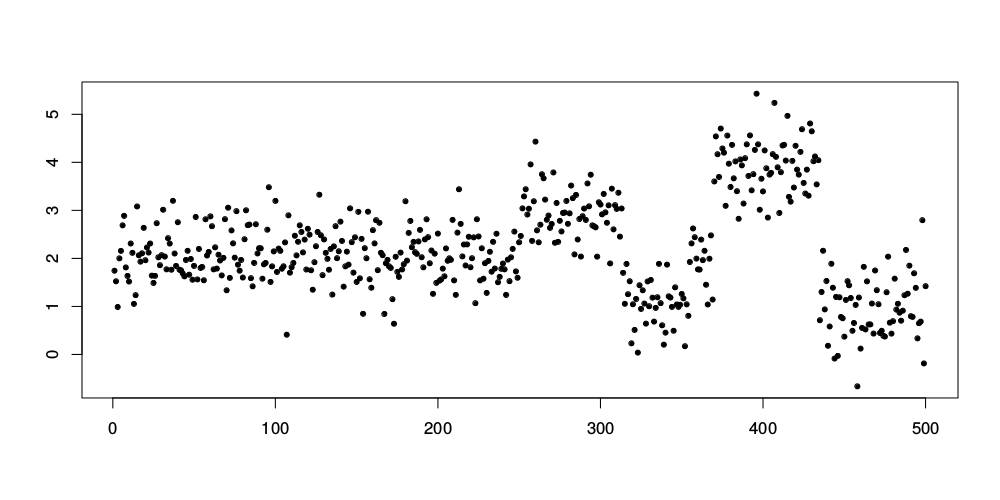
\includegraphics[height=.45\textheight, width=.9\textwidth]{../Figures/FigSeg-Cambridge-CGH}
	   \onslide<2>
	   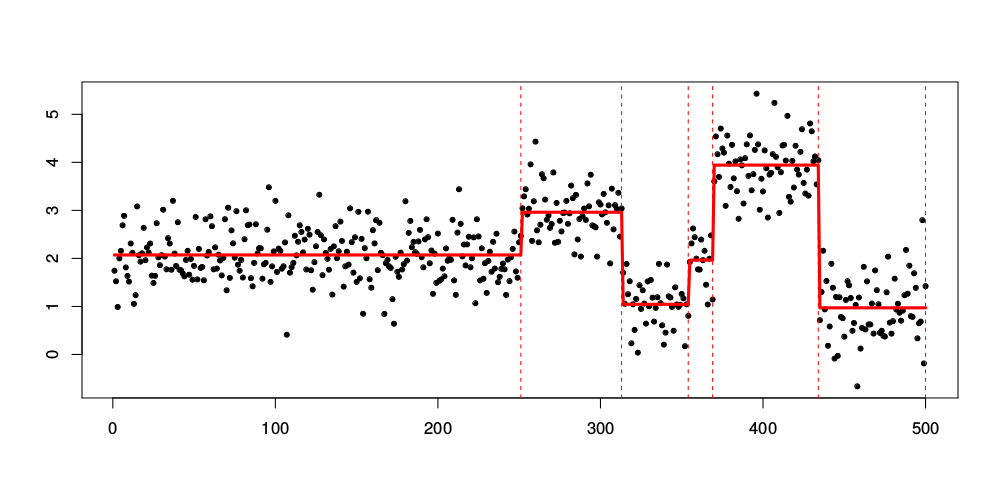
\includegraphics[height=.45\textheight, width=.9\textwidth]{../Figures/FigSeg-Cambridge-CGH-seg}
	 \end{overprint}
    \end{tabular}
    \\
    \vspace{-.05\textheight}
    \paragraph{RNA-sequencing:} massive sequencing / gene expression \\
    \begin{tabular}{c}
	 \begin{overprint}
	   \onslide<1>
	   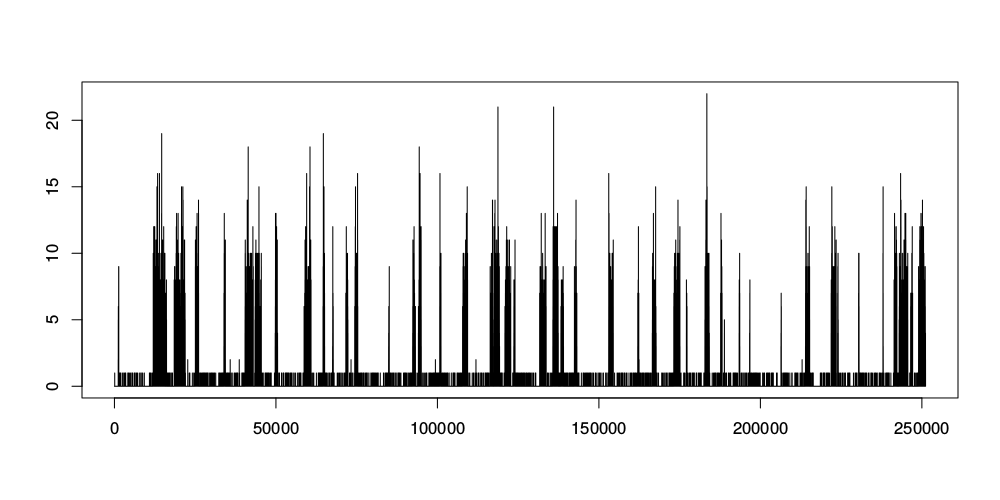
\includegraphics[height=.45\textheight, width=.9\textwidth]{../Figures/FigSeg-Cambridge-RNAseq}
	   \onslide<2>
	   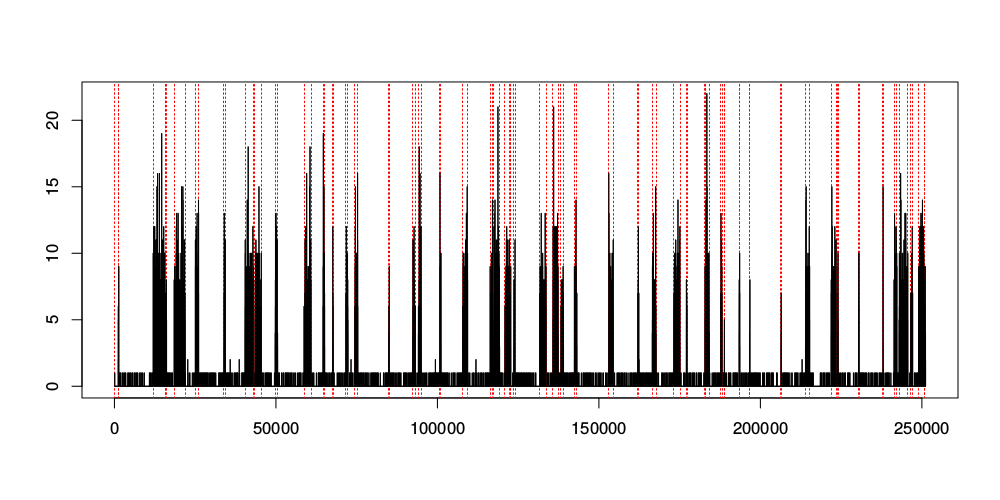
\includegraphics[height=.45\textheight, width=.9\textwidth]{../Figures/FigSeg-Cambridge-RNAseq-seg}
    \end{overprint}
    \end{tabular}
  \end{tabular}
  }

%====================================================================
\frame{\frametitle{CNV detection using microrray}

  $$
  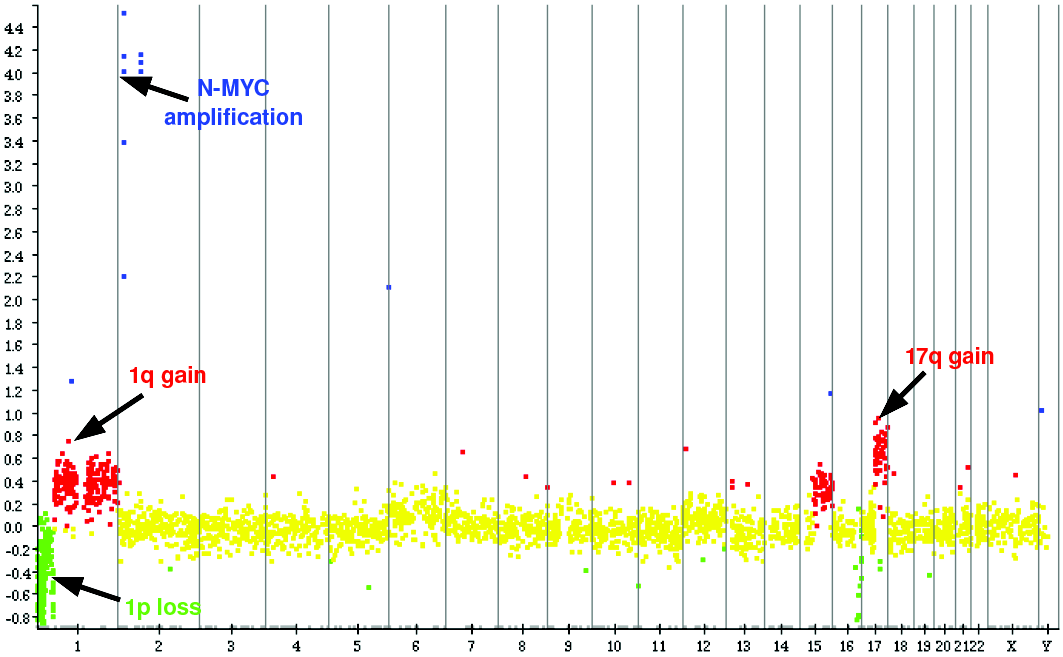
\includegraphics[height=.5\textheight, bbllx=80, bblly=617, bburx=150, bbury=700]{../Figures/Hup08-Fig128a}
  $$
  \refer{Hup08}
  
  
  \bigskip
  \paragraph{Data.}
  $$
  Y_t = \text{log-fluoresence ratio at probe $t$}
  $$	
}

%====================================================================
\frame{\frametitle{Example: Breast cancer CGHarray}

  \vspace{-.5cm}
  \[
  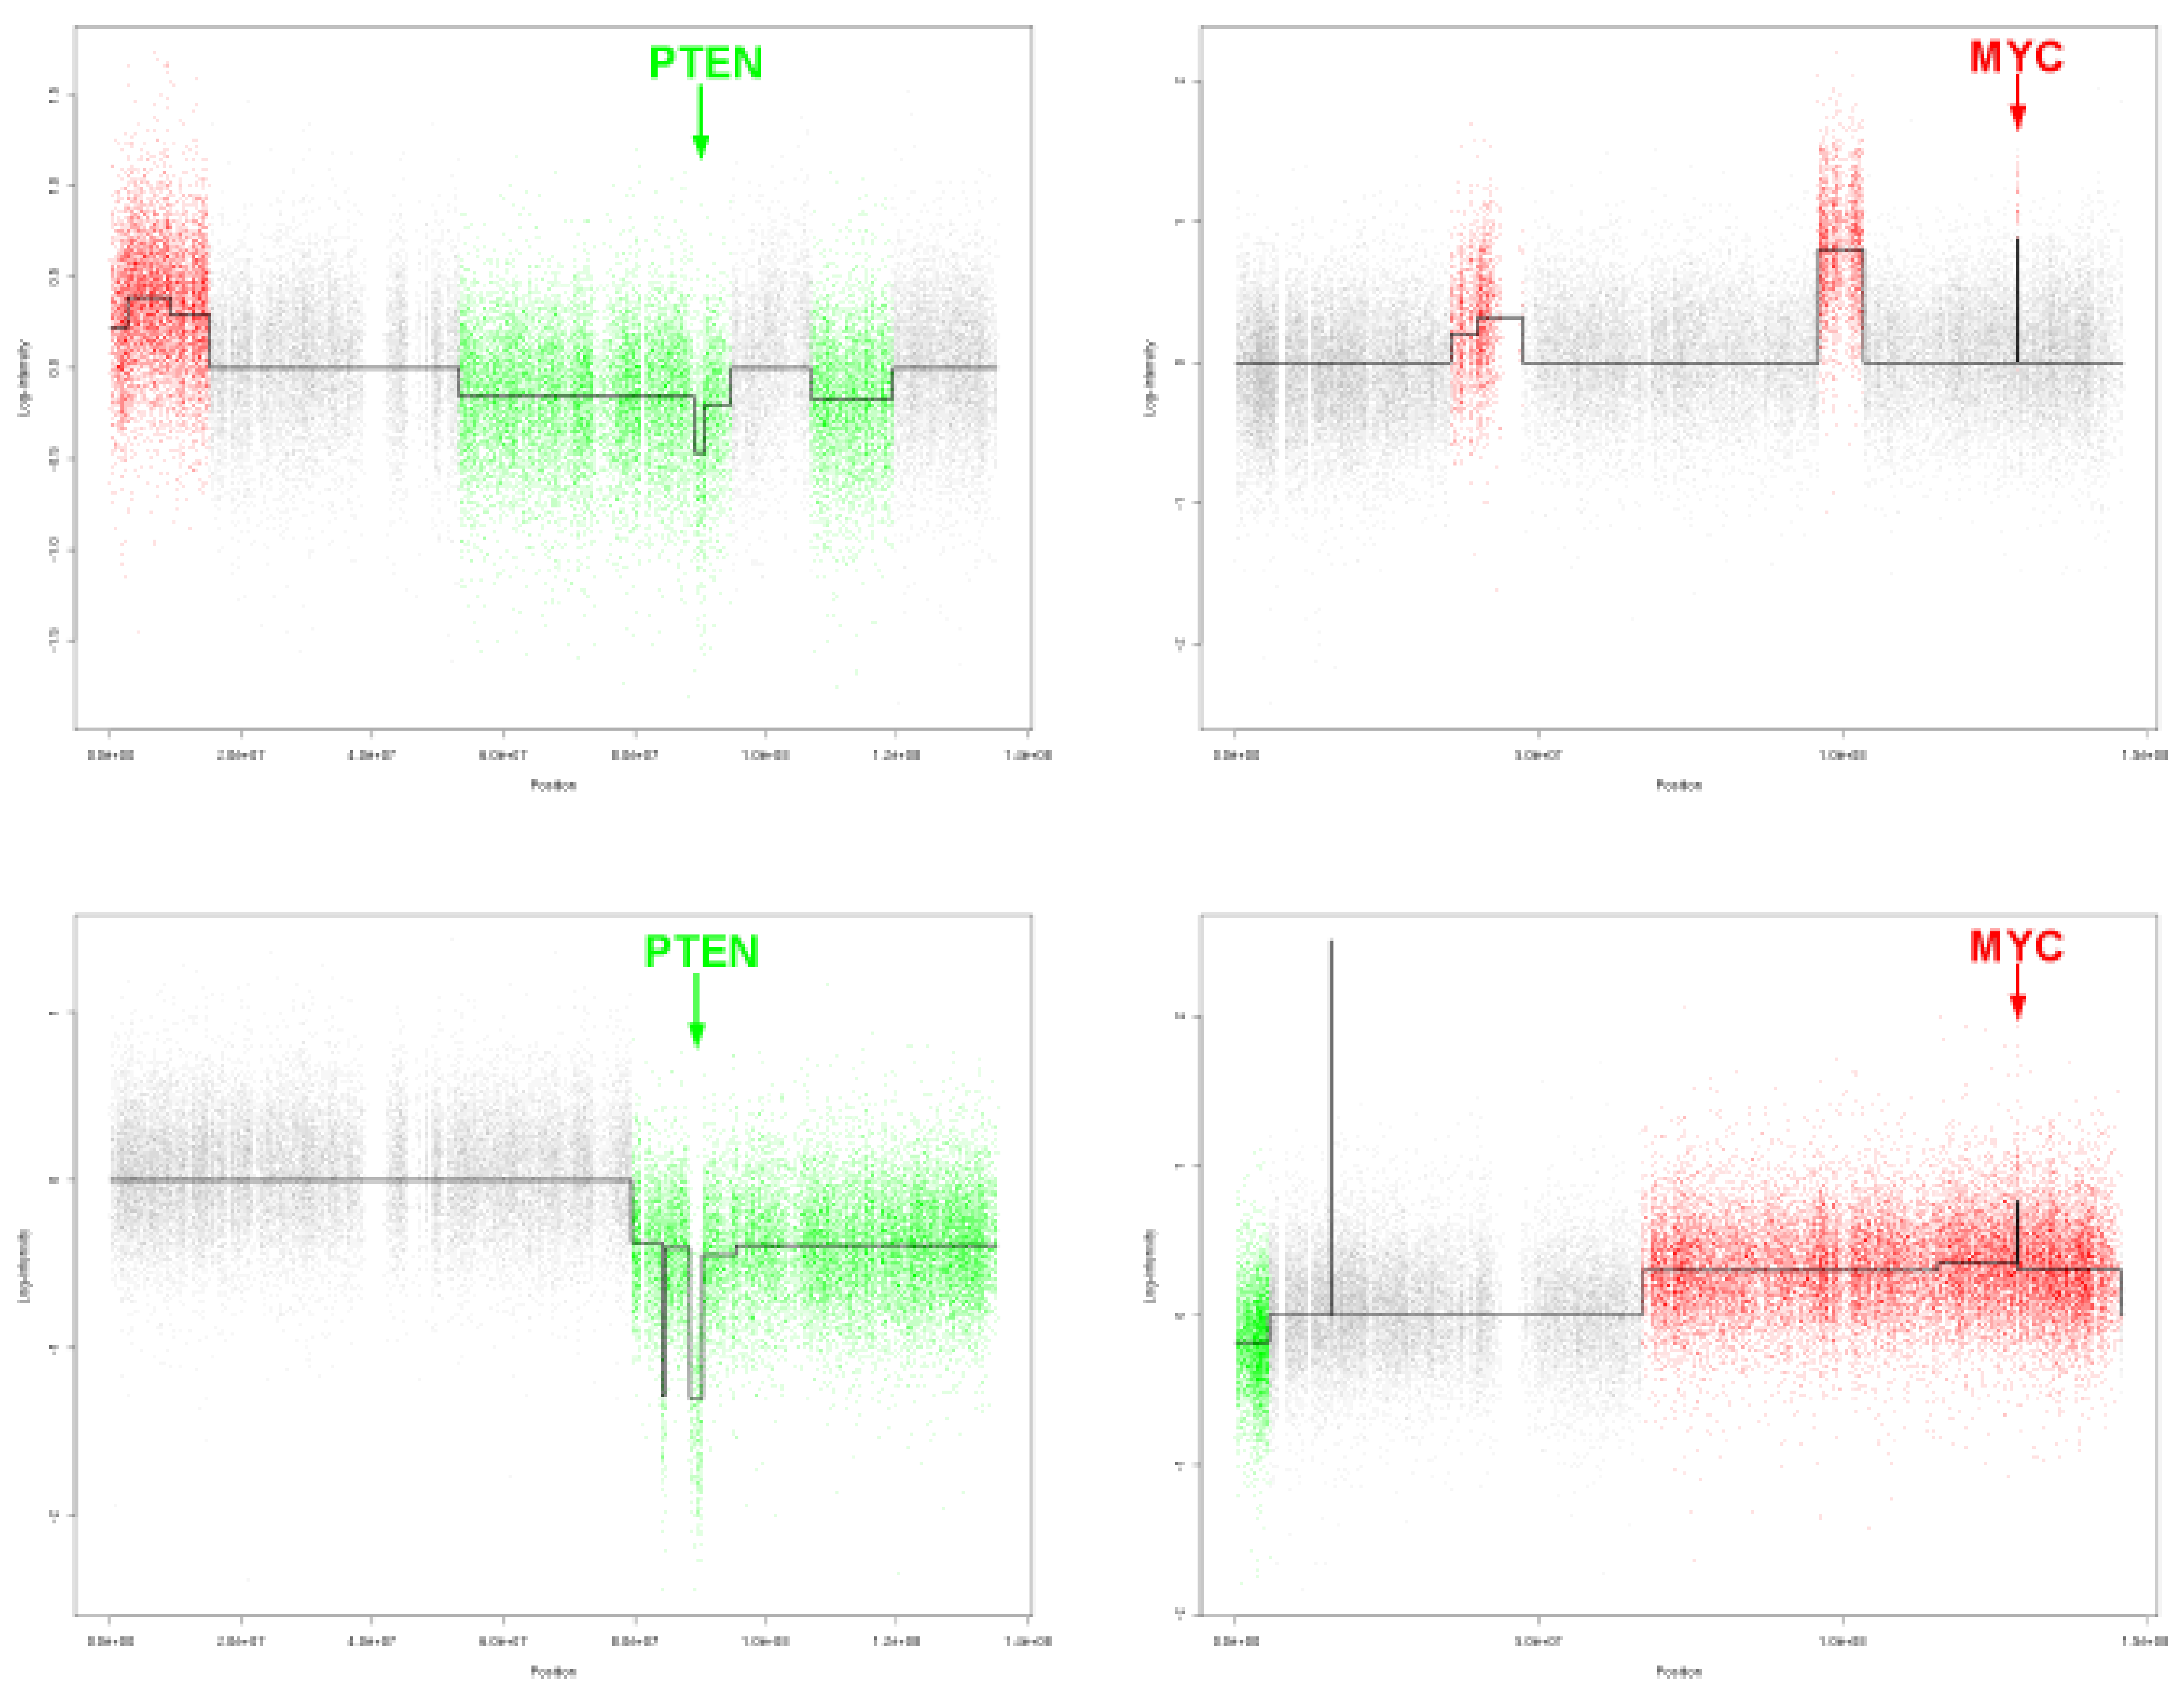
\includegraphics[height=.8\textheight, width=.8\textwidth]{../Figures/Rig10-Fig6-5} 
  \] 
  Chrom. 10 and 8 of two breast carcinomas (TNBC). \refer{Rig11} 
}\label{Page:BreastCancer}

%====================================================================
\frame{\frametitle{Gene discovery with RNA-seq}

  \paragraph{Data:} $Y_t =$ number of reads mapped onto the genome and starting at nucleotide $t$

  $$
  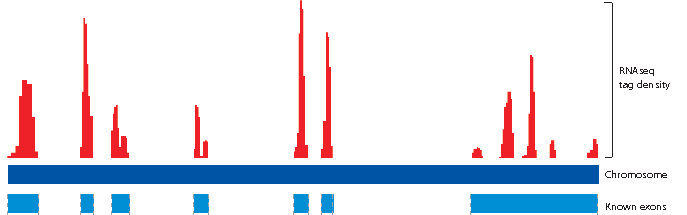
\includegraphics[width=.8\textwidth, height=.4\textheight]{../Figures/gb-2008-9-9-234-1}
  $$
  \Refer{genomebiology.com}
  
  \bigskip \bigskip 
  \paragraph{Aim:} Determine the boundaries of the transcribed regions.

}

%====================================================================
\frame{\frametitle{Three main issues} 

  \paragraph{Modelling}
  \begin{itemize}
   \item Which distribution: Gaussian, Poisson, negative Binomial?
   \item Independence?
  \end{itemize}
  
  \bigskip 
  \paragraph{Algorithmics:} $\binom{n-1}{K-1} \approx \left(\frac{n}{k}\right)^k$ possible segmentations of $n$ points into $K$ segments
  \begin{description}
  \item[\ra] Dynamic programming retrieves the optimal segmentation in $O(Kn^2)$ for additive loss functions
  \end{description}
  
  
  \bigskip 
  \paragraph{Model selection:} How many segments: $K = $ ?
  \begin{description}
   \item[\ra] Because of discontinuity, standard model selection criteria (AIC, BIC) do not apply
  \end{description}

  }

%====================================================================
\frame{\frametitle{Two scales} 

  \paragraph{Global scale: $n \approx 10^6 - 10^8$} (whole genome) \\
  Aim = find the 'best' segmentation, not much more.
  \begin{itemize}
   \item Need for efficient algorithms %(not quadratic!) \\
%    \ra P. Fearnhead's \refer{KFE12} and G. Rigaill's \refer{Rig10} talk on January 16th
   \item Need for a dedicated criterion to choose $K$: %see \refer{ClL13}\\
%    $+$ D. Siegmund's talk on January 13th  \refer{ZhS07} 
  \end{itemize}

  \bigskip \bigskip 
  \paragraph{Local scale: $n \approx 10^3$} (genomic region) \\
  Aim = answer to more precise questions
  \begin{itemize}
   \item Reliability of the 'best' segmentation
   \item Confidence intervals for the change points
   \item Change point comparison
  \end{itemize}
  }


% %====================================================================
% \frame{\frametitle{Global scale: comparative study for SNP arrays}
% 
%   \paragraph{Benchmark of manually annotated profiles:} ROC curves \refer{Hoc12}
%   $$
%   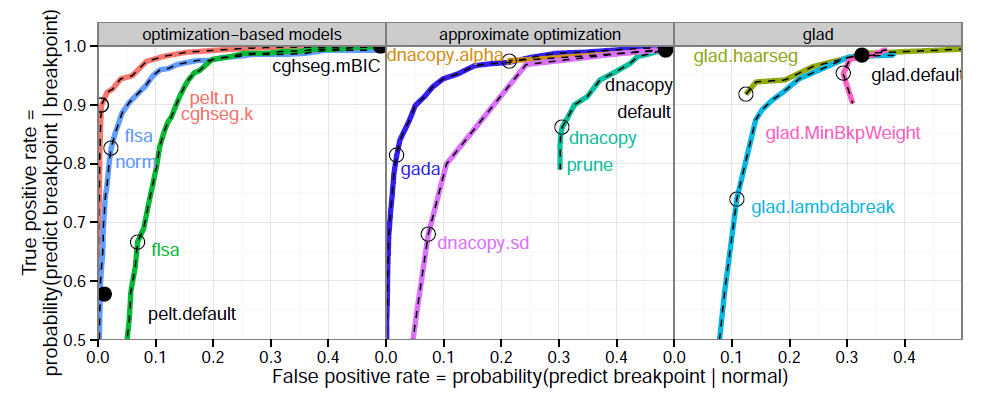
\includegraphics[width=\textwidth]{../Figures/Hoc12-Fig3-3}     
%   $$
% %   \begin{itemize}
% %    \item 'Exact' methods (PDPA \refer{Rig10} and PELT \refer{KFE12}) perform best 
% %    \item Model selection remains an issue.
% %   \end{itemize}
% 
%  }

% %====================================================================
% \frame{\frametitle{Change-point detection in genomics} 
% %====================================================================
%   Change-point (or segmentation) problems raise in many fields of genomics:
%   \begin{itemize}
%    \item Copy number variation (CGHarrays, DNAseq),
%    \item Gene detection (tilling arrays, RNA-seq),
%    \item Protein-DNA interaction (ChIP-chip, CHiP-seq),
%    \item and many others...
%   \end{itemize}
% 
%   \bigskip \bigskip \pause
%   They are faced as soon as one deal with data
%   \begin{itemize}
%    \item organized along one dimension (time, genome position, ...),
%    \item expected to display abrupt changes,
%    \item in presence of noise.
%   \end{itemize}
% }
%====================================================================

%====================================================================
\subsection*{Examples}
% %====================================================================
% \frame{\frametitle{CNV analysis with DNAseq}
% 
%   \begin{itemize}
%    \item DNAseq reads are mapped along a reference genome. 
%    \item Variation of there density reveals variation of the copy number.
%   \end{itemize}
% 
%   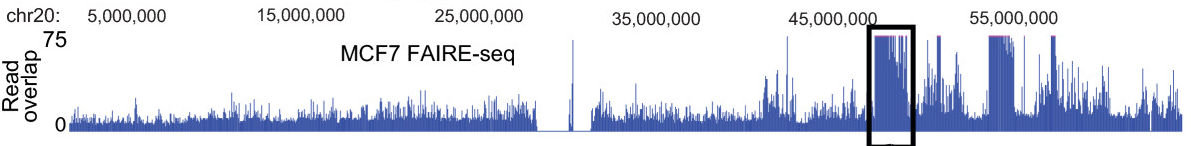
\includegraphics[width=.9\textwidth]{../Figures/RGI12-Fig4c} 
%   \\
%   \refer{RGI12}
% 
%   \bigskip \bigskip
%   \paragraph{Data.}
%   $$
%   Y_t = \text{number of mapped reads starting at nucleotide $t$}
%   $$	
%   \ra 'depth of coverage', 'read depth'.
%   }
% 
%====================================================================
\subsection*{(Statistical) questions}
%====================================================================
\frame{\frametitle{Segmentation: the basic problem}
  
  %\vspace{-0.5cm}
  \begin{tabular}{cc}
    \begin{tabular}{p{.5\textwidth}}
      \onslide+<1->{
        \paragraph{Data at hand:} for a given individual
        \begin{itemize}
        \item a sequence of {known positions} along the
          {reference genome}, labeled as
          \[
          t = 1, 2, \dots, n
          \]
        \item a signal measured {at each position}
          \[
          Y_t = \text{signal at position $t$}
          \]
        \end{itemize}
        }
    \end{tabular}
    &
    \begin{tabular}{p{.5\textwidth}}
      \hspace{-1cm}
      \begin{overprint}
        \onslide<2-3>
        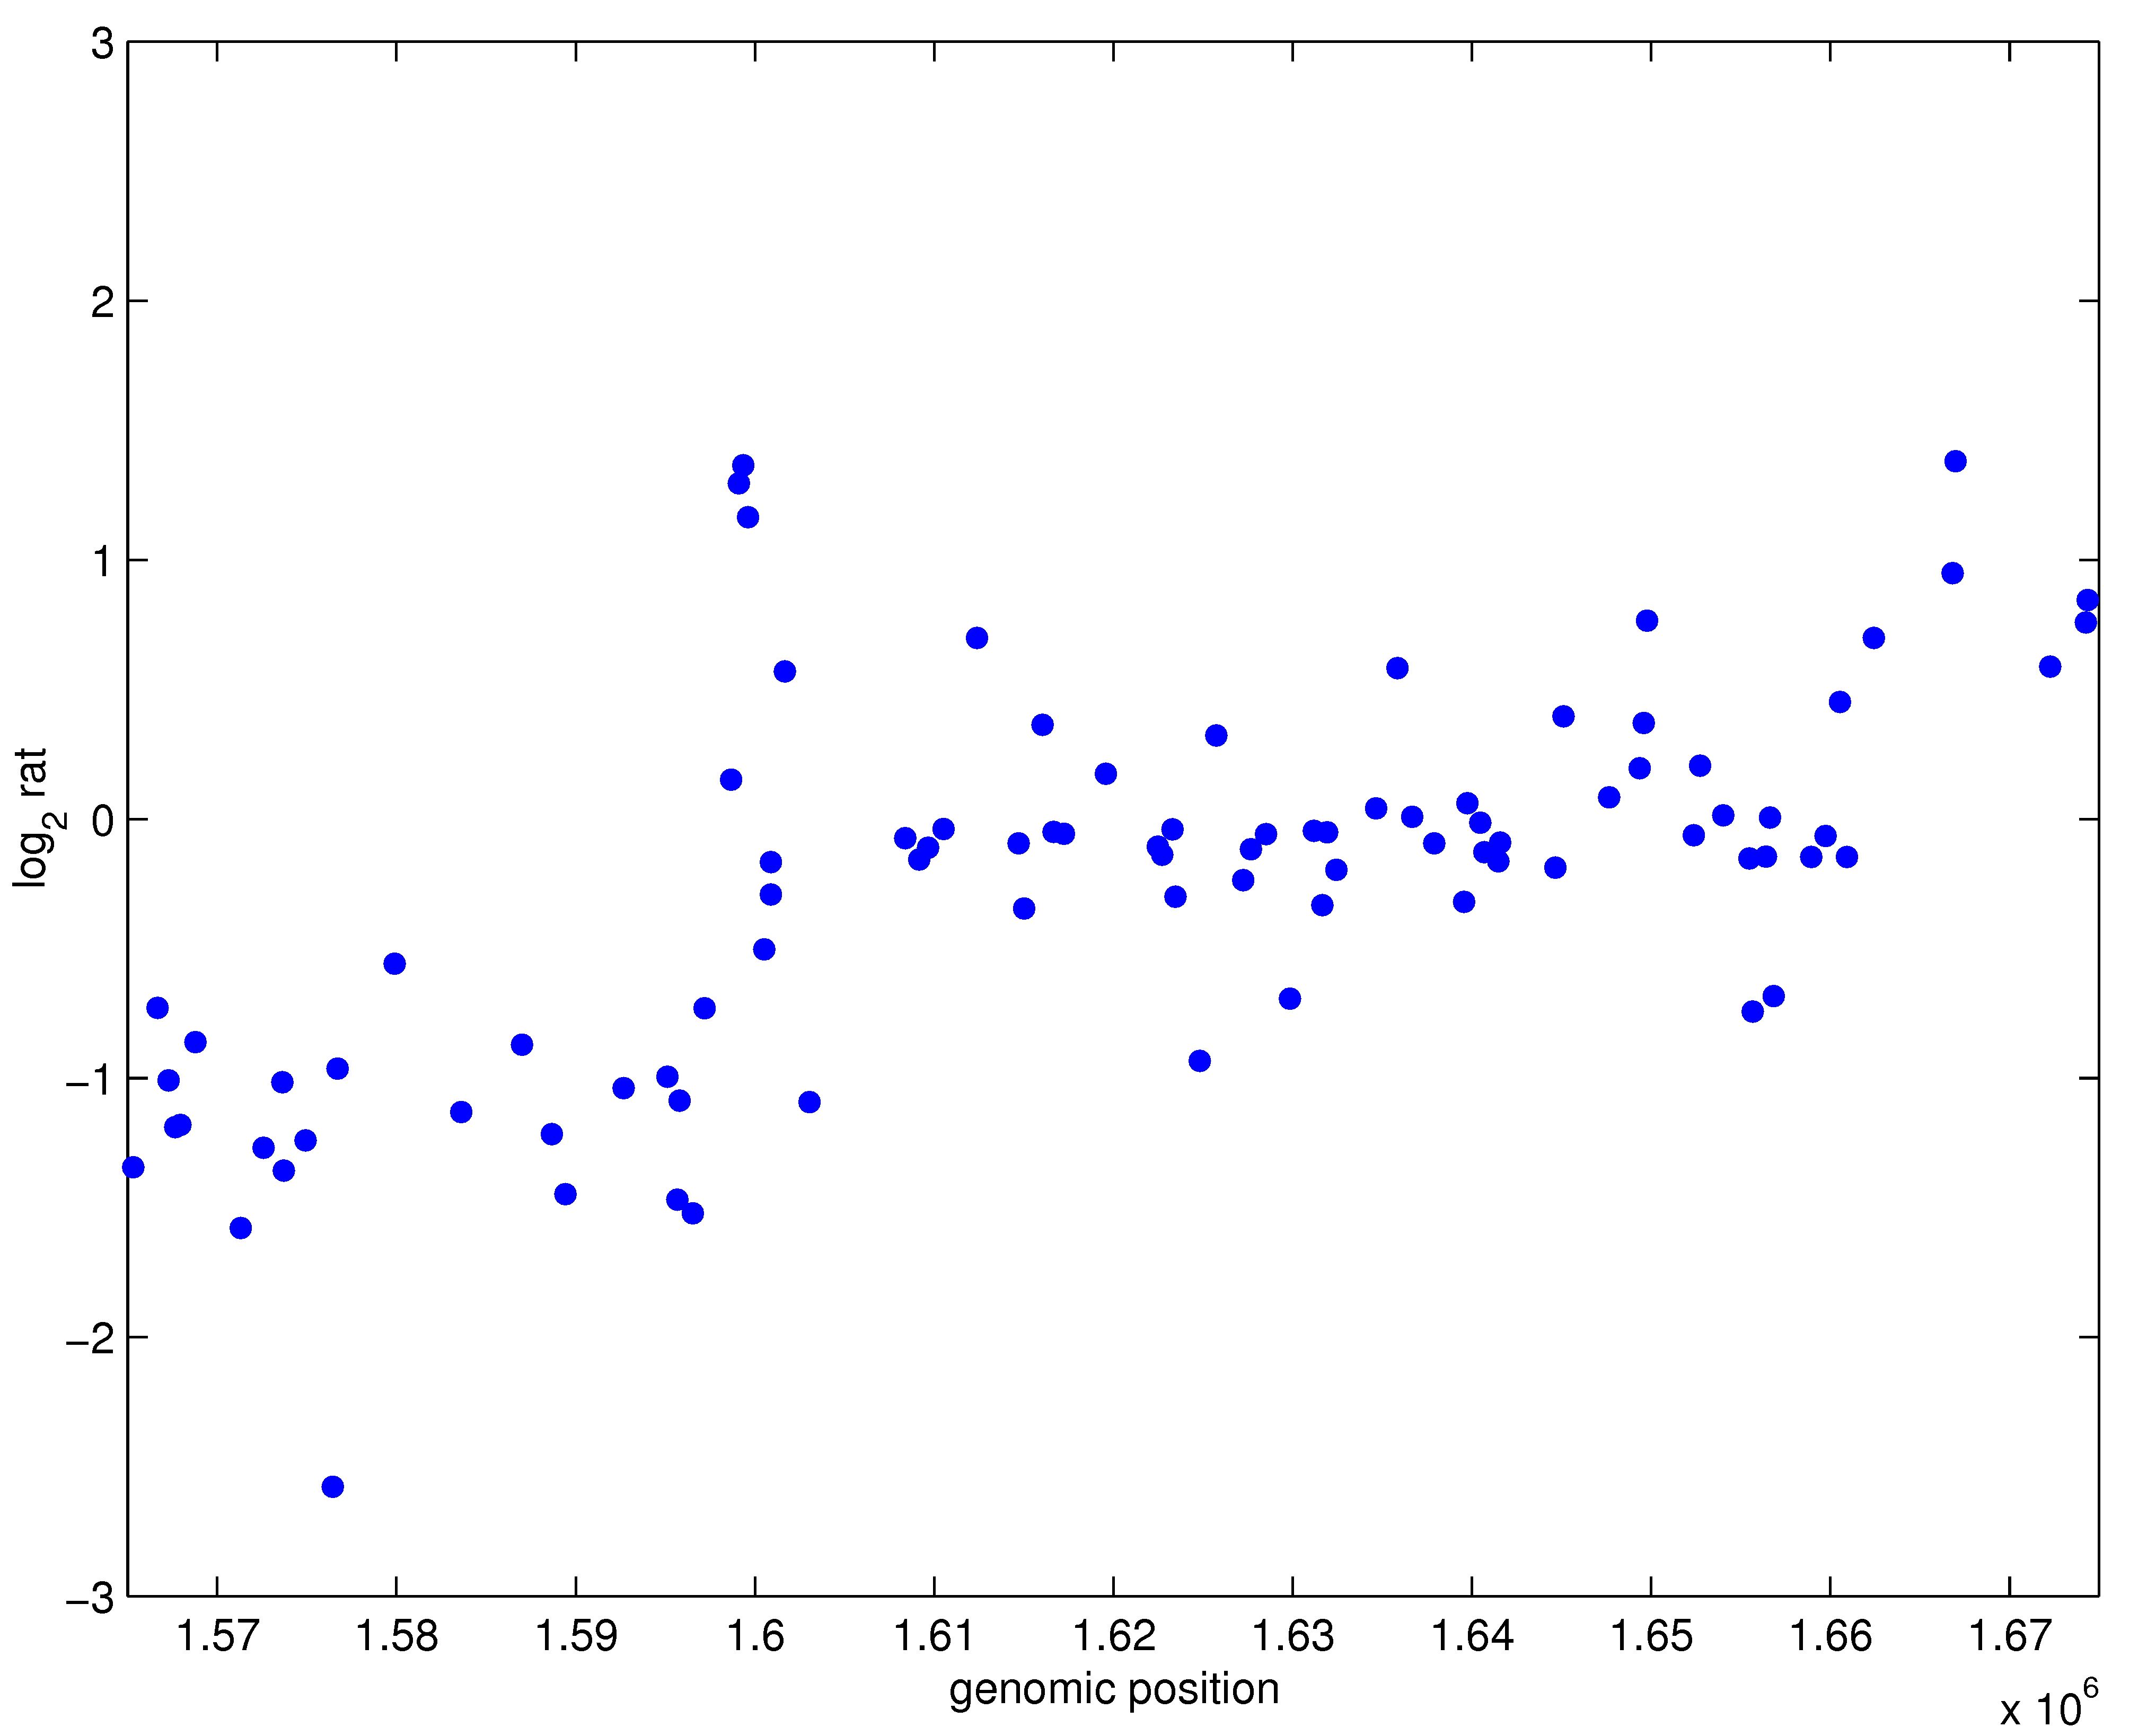
\includegraphics[width=.45\textwidth, height=.5\textheight]{../Figures/raw_profile_example} 
        \onslide<4>
        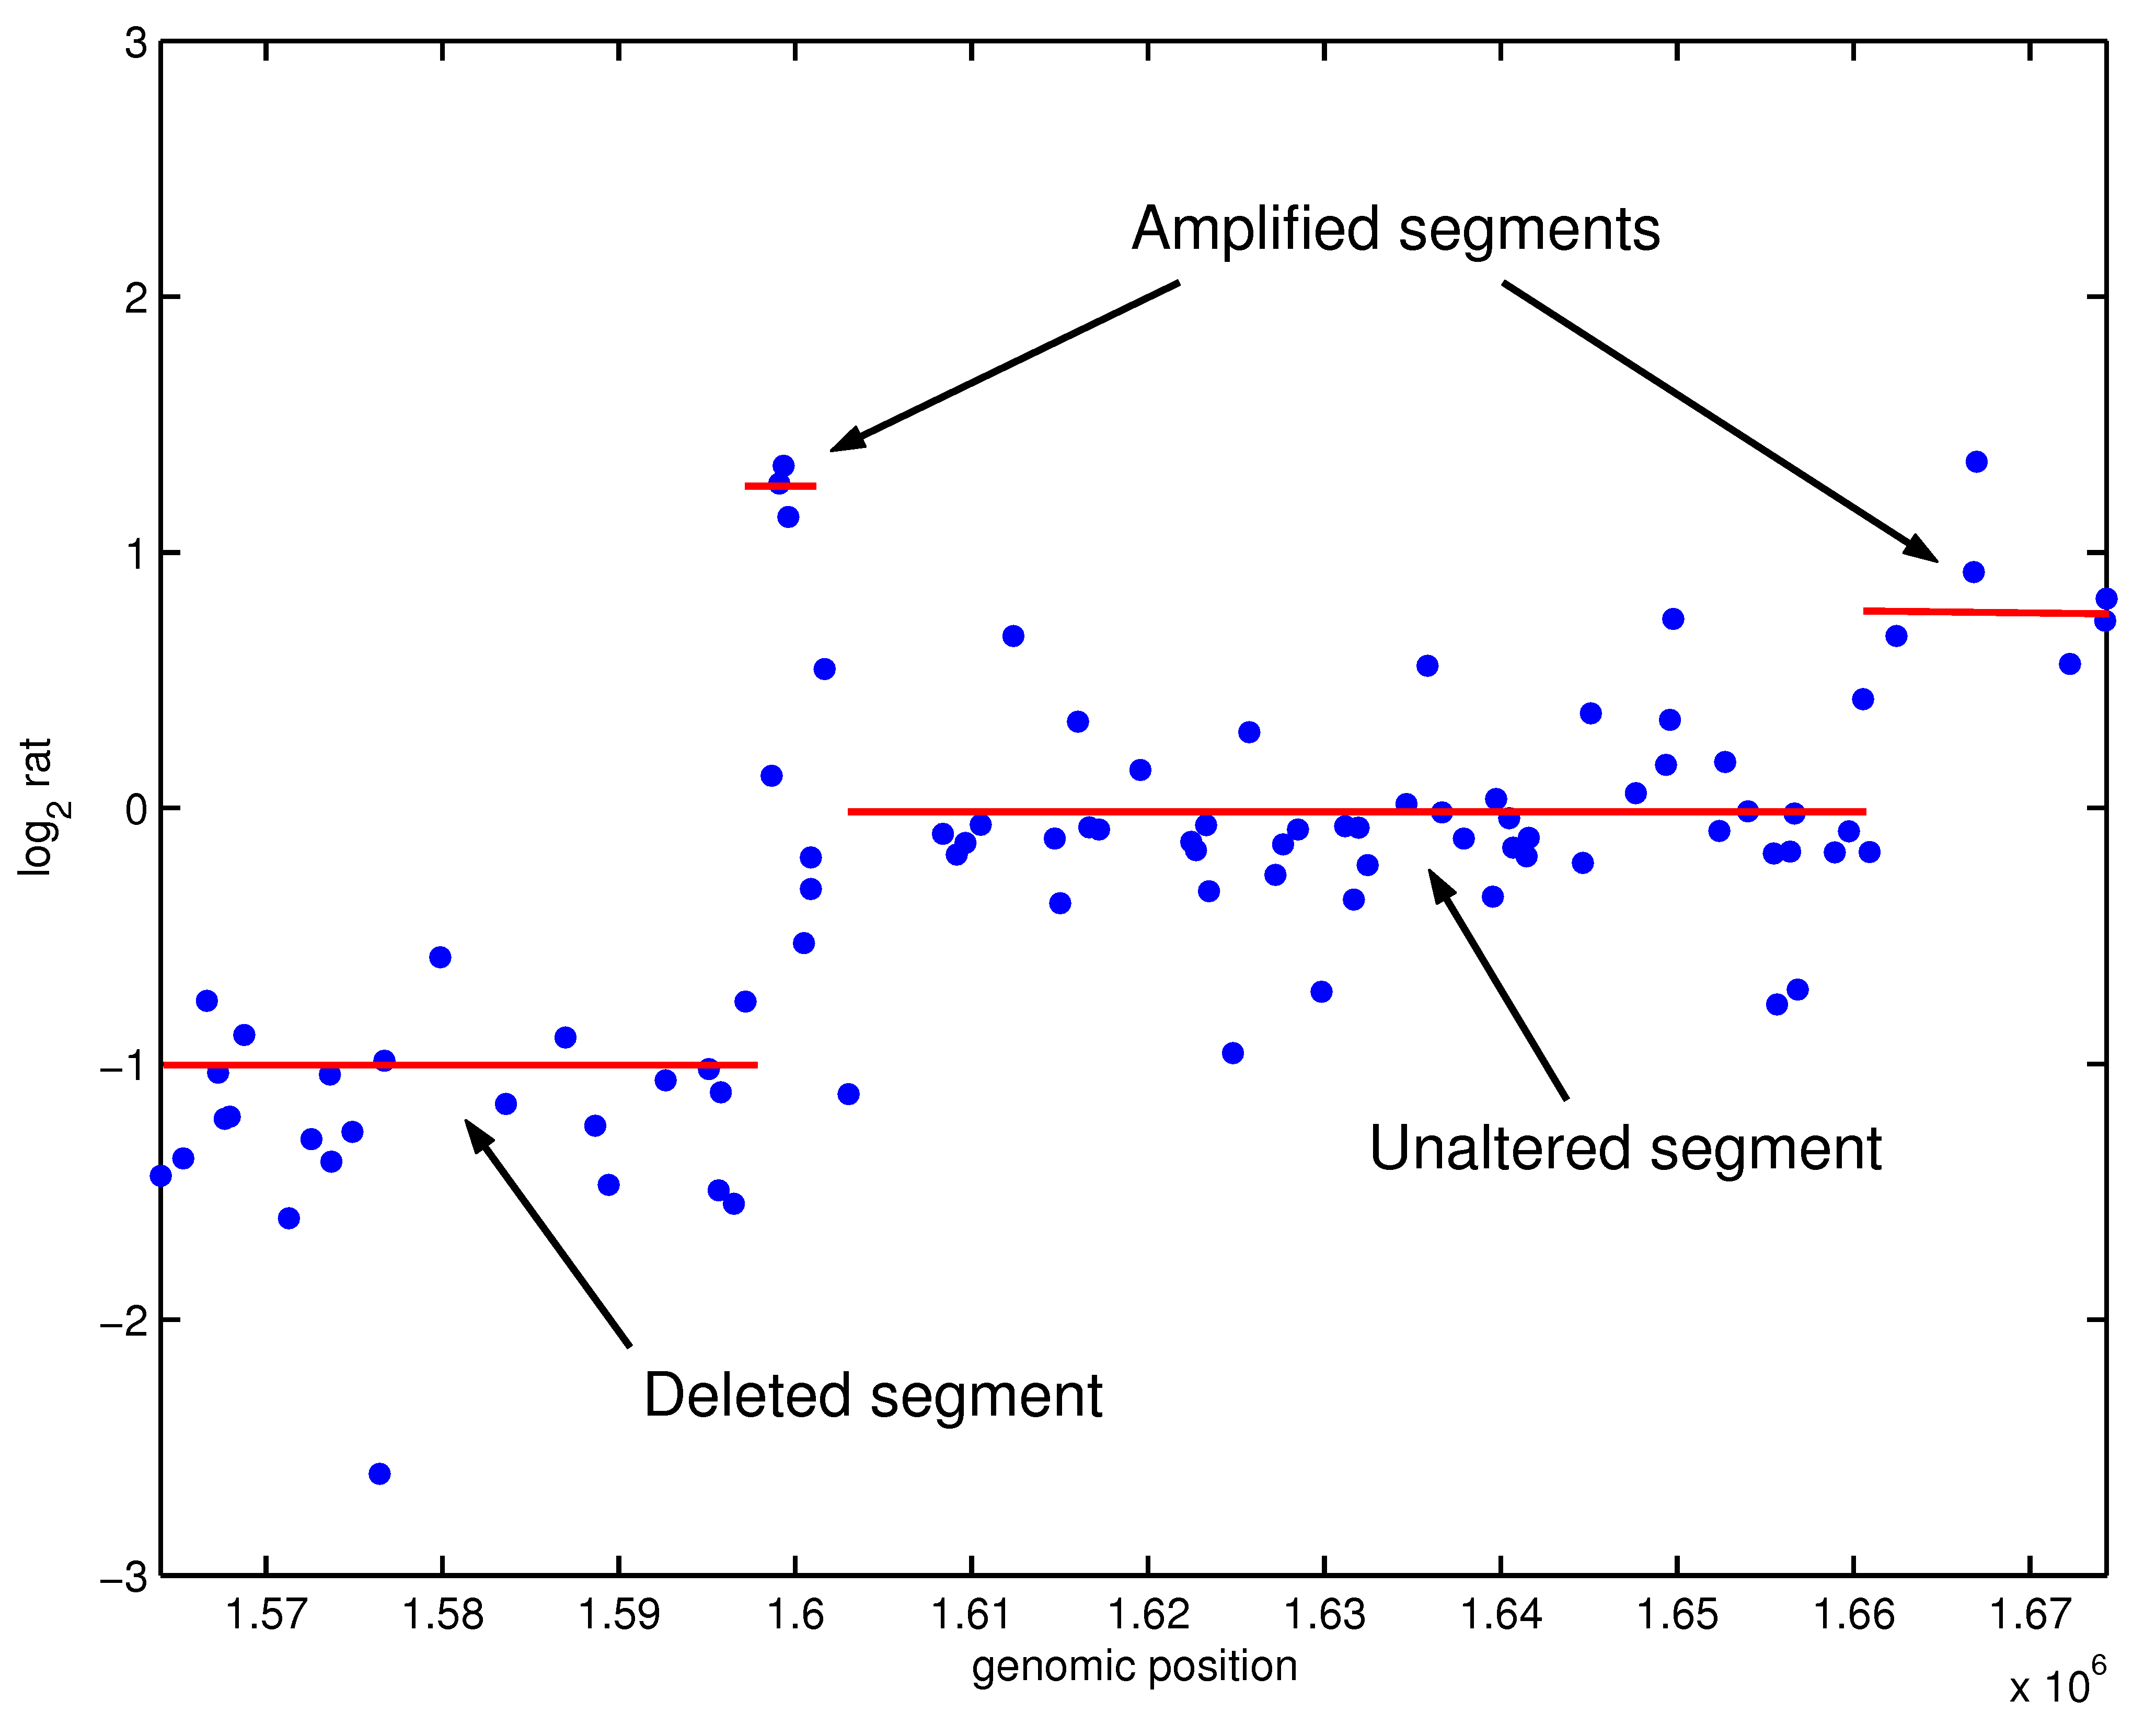
\includegraphics[width=.45\textwidth, height=.5\textheight]{../Figures/profile_example}
      \end{overprint}
    \end{tabular}
  \end{tabular} \\
  \onslide+<3->{
    \begin{eqnarray*}
      Y_t & \propto & f(\text{{relative copy number} at position }t) \\
      & = & \text{DNAseq count, log-fluorescence, etc.}
    \end{eqnarray*}
    }
  }

%====================================================================
\frame{\frametitle{(Statistical) questions}
  
  \paragraph{Biological questions:}  
  \begin{itemize}
  \item How many change-points?
  \item Where are the change-points? (How precise is the location?)
  \item Do the change-points have the same location in samples $A$
    and $B$?
  \item ...
  \end{itemize}
  
  \bigskip\pause
  \paragraph{Statistical issues:}  
  \begin{itemize}
  \item Statistical modeling
  \item Computational efficiency
  \item Model selection
  \item Model comparison
  \end{itemize}
}

% %====================================================================
% \frame{\frametitle{Data specificities}
% 
%   \paragraph{Dimension.}
%   \begin{itemize}
%    \item Whole chromosome CNV detection using DNAseq \ra $n = 10^8$
%    \item Whole chromosome CNV detection using SNParray \ra $n = 10^6$
%    \item 'Small' gene reannotation  using RNAseq \ra $n = 10^4$
%   \end{itemize}
%   \ra Different computational burdens.
% 
%   \bigskip \pause
%   \paragraph{Stucture.}
%   \begin{itemize}
%    \item One measurement per position (probe or nucleotide)
%    \item Pairs of positions (pair-end) \ra \emphase{out of my scope}\footnote{Are statisticians slower than computer scientists?}
%   \end{itemize}
%   
%   \bigskip \pause
%   \paragraph{Nature.}
%   \begin{itemize}
%    \item Microarray \ra fluorescence \ra continuous data ($\in \Rbb$)
%    \item NGS \ra read counts \ra discrete data ($\in \mathbb{N}$)
%   \end{itemize}
% 
% }

%====================================================================
%====================================================================
\section{Segmentation methods}
\frame{\frametitle{Segmentation methods}}
%====================================================================

%====================================================================
\subsection*{Statistical model} 
% ====================================================================
% \frame{\frametitle{A model, what for?} 
%   
%   \begin{itemize}
%   \item To {translate biological questions into mathematical
%       equations} and quantities;
%   \item To make {all hypotheses explicit};
%   \item To set the inference of interesting parameters in a
%     {global framework}, possibly accounting for other effects
%     (covariates);
%   \item To {motivate all calculations} and data processing to
%     come.
%   \end{itemize}
%   
%   \bigskip\pause
%   \centerline{\sl The model is the place where biologist's and mathematician's minds meet.}
%   
%   \bigskip\bigskip\pause
%   \paragraph{Model-based approach.}
%   \begin{itemize}
%   \item Define a model that describes the biological process as well
%     as possible;
%   \item Make sure that it can be handled in terms of mathematics /
%     statistics;
%   \item Derive an (efficient and statistically valid) inference
%     procedure.
%   \end{itemize}
% }
% 
%====================================================================
\frame{\frametitle{Segmentation model}

  \begin{tabular}{cc}
    \hspace{-.5cm}
    \begin{tabular}{p{.5\textwidth}}
      \onslide+<2->{\paragraph{Statistical model.} 
        \begin{itemize}
        \item $\text{Signal} = f(\text{Position})$; \\}
        \onslide+<3->{
        \item Breakpoint positions: \\
          $\tau_1, \tau_2, ..., \tau_{K-1};$ \\}
        \onslide+<4->{
        \item 'Mean' signal (e.g. copy number) within each interval: \\
          $\mu_1, \mu_2, ..., \mu_K$; \\}
        \onslide+<5->{
        \item Observed signal at time $t$: \\
          independent variables with given parameter (mean, dispersion, ...).
        \end{itemize}}
    \end{tabular}
    & 
    \hspace{-1cm}
    \begin{tabular}{c}
      \onslide+<2->{
        \hspace{-6cm}
        \onslide+<3->{if $t \in \textcolor{blue}{r_k}$,} \quad $Y_t$
        \onslide+<5->{$\sim
          \Fcal($}\onslide+<4->{$\textcolor{red}{\mu_k}$}\onslide+<5->{$)$}
        \\}
      \begin{overprint}
        \onslide<2>
%        $\qquad \qquad \;\;\, Y_t =$ \\
        \includegraphics[width=.5\textwidth]{../Figures/FigSeg-Budapest-1} 
        \onslide<3>
%        if $t \in \textcolor{blue}{r_k}, \quad Y_t$ \\
        \includegraphics[width=.5\textwidth]{../Figures/FigSeg-Budapest-2} 
        \onslide<4>
%        if $t \in \textcolor{blue}{r_k}, \quad Y_t \textcolor{red}{\mu_k}$ \\
        \includegraphics[width=.5\textwidth]{../Figures/FigSeg-Budapest-3} 
        \onslide<5->
%        if $t \in \textcolor{blue}{r_k}, \quad Y_t \sim
%        \Fcal(\textcolor{red}{\mu_k})$ \\ 
        \includegraphics[width=.5\textwidth]{../Figures/FigSeg-Budapest-4} 
      \end{overprint}
    \end{tabular}
  \end{tabular}

%   \onslide+<6->{
%     \paragraph{Possible choices for the distribution $\Fcal$:} 
%     \begin{itemize}
%     \item CGHarray: continuous signal (fluorescence) \ra Gaussian distribution;
%     \item NGS: discrete signal (counts) \ra Poisson or negative
%       binomial distribution.
%     \end{itemize}
%   }
}

%====================================================================
\frame{\frametitle{Dealing with (some) data specificities} 
  
  \paragraph{Distribution.} The distribution $\Fcal$ of the data is chosen according to the technology:
    $$
    \begin{array}{c}
      \text{if position $t$} \\
      \text{is in segments $r_k$:}
    \end{array}
    \quad 
    \left\{ 
      \begin{array}{rcll}
        Y_t & \sim & \Ncal(\mu_k,\sigma^2)  & \text{aCGH (same
          variance)} \\
        \\
%         Y_t & \sim & \Ncal(\mu_k,\sigma_k^2)  & \text{aCGH (heter.
%           variance)} \\  
%         \\
        Y_t & \sim & \Pcal(\mu_k)  &  \text{NGS} \\
        \\
        Y_t & \sim & \Ncal\Bcal(\mu_k, \phi)  &  \text{NGS (over-dispersed)}
      \end{array}
    \right.
    $$

%     \bigskip \pause
%     \paragraph{Normalization?}
%     {Explicit modeling allows to account for additional information}, e.g. $x_t =$ GC content at position $t$:
%     $$
%     Y_t \sim \Ncal(\mu_k + \lambda x_t, \sigma^2)
%     $$	
%     (see CGHseg package later on).
  }

% %====================================================================
% \frame{\frametitle{Data transformation}
% 
%   \begin{itemize}
%   \item The reference distributions for NGS data are Poisson and negative binomial for which many methods are being developped. \\~ \\
%   \item \pause Many methods exist for continuous data (Gaussian, as usual, easier to handle). \\~ \\
%   \item \pause Data transformation could be used to apply them to NGS data, e.g.:
%   $$
%   \widetilde{Y}_t = \log(1 +  Y_t), 
%   \qquad
%   \widetilde{Y}_t = \sqrt{Y_t}, 
%   $$ \\
%   \item \pause Reminder: the variance stabilizing transformation for the negative binomial is 
%   $$
%   \widetilde{Y}_t = \arg \sinh \sqrt{{Y_t}/{\phi}}
%   $$	
%   \end{itemize}
% }

%====================================================================
\subsection*{Parameter inference}
%====================================================================
\frame{\frametitle{Parameter inference}

  \paragraph{Two different types of parameters of the models:}
  \begin{itemize}
  \item Segmentation (change-point locations): $T = (\tau_1, \dots,
    \tau_{K-1})$ \\
    \ra discrete parameter;
  \item Distribution parameters (within segment means): $\mubf =
    (\mu_1, \dots, \mu_K)$ \\
    \ra continuous parameter.
  \end{itemize}

  \bigskip\bigskip\pause
  \paragraph{Fitting model to data:} The estimates of $T$ and $\mu$ are expected to provide a good fit to the data.
  \begin{enumerate}
   \item Define a criterion to measure this fit
   \item Find the 'optimal' values $\widehat{T}$ and $\widehat{\mubf}$ providing the best fit.
  \end{enumerate}

}

%====================================================================
\frame{\frametitle{Maximum likelihood}

  \paragraph{Most common strategy: Maximum likelihood.}
  To get estimate of the parameters of this model ($T, \mubf$)
  we choose to maximize the likelihood of the observed data:
  \begin{eqnarray*}
  p(\Ybf; T, \mubf) & = & \textcolor{red}{\prod_k} \textcolor{blue}{\prod_{t \in r_k}} p(Y_t; \mu_k) \\
  \Rightarrow \qquad \log p(\Ybf; T, \mubf) & = & \textcolor{red}{\sum_k}
  \textcolor{blue}{\sum_{t \in r_k}} \log p(Y_t ;\mu_k).
  \end{eqnarray*}

  \bigskip\pause
  \paragraph{Array CGH.} Gaussian with same variance $\Ncal(\mu_k, \sigma^2)$:
  $$
  \log P(\Ybf; T, \mubf) = \text{cst} - \text{cst} \sum_k \sum_{t \in r_k} (Y_t - \mu_k)^2
  $$
  
  \bigskip\pause  
  \paragraph{NGS.} Poisson $\Pcal(\mu_k)$:
  $$
  \log P(\Ybf; T, \mubf) = \text{cst} - \sum_k \sum_{t \in r_k}
  (\mu_k - Y_t \log \mu_k)
  $$

  }
  
%====================================================================
\frame{\frametitle{Parameter inference} 

  \paragraph{When the breakpoints are known,} estimating the
  parameters is (generally) an easy task, e.g. for the mean
  $$
  \widehat{\mu}_k = \frac1{n_k} \sum_{t \in r_k} Y_t
  $$

  \pause\bigskip
  \paragraph{Finding the breakpoints:} We now have to find the change-points $T = (\tau_1, \dots, \tau_{K-1})$ that maximize the log-likelihood
  $$
  \log p(\Ybf; T) = \sum_k  \sum_{t \in r_k} \log p(Y_t ;\widehat{\mu}_k).
  $$
  \pause\bigskip
  \paragraph{Problem.} There are $ \binom{n-1}{K-1} $ possible choices
  for the positions of the breakpoints $\tau_1, \tau_2, \dots,
  \tau_{K-1}$.
  $$
  \text{For } n=1\,000, \qquad K = 20 \quad \longrightarrow \quad
  \binom{n-1}{K-1} \simeq 10^{40}
  $$
  \ra Impossible to explore for large $n$ and $K$

}\label{Page:ParamInfer}

%====================================================================
\subsection*{Dynamic programming}
%====================================================================
%====================================================================
\frame{\frametitle{Shortest path problem}

  \paragraph{Cost of segment.} Define the cost of segment $r= [i, j]$ as
  $$
  C(i, j) = \sum_{t \in [i, j]} - \log p(Y_t; \widehat{\mu}_{[i, j]}),    
  $$
  finding the maximum likelihood segments
%   the maximization of
%   $$
%   \log p(\Ybf; T) = \sum_k  \sum_{t \in r_k} \log p(Y_t; \widehat{\mu}_k).
%   $$
  can be restated as a \paragraph{shortest path problem}, that is to find the path
  \begin{itemize}
  \item going from 1 to $n$,
  \item in $K$ steps,
  \item for the best possible cost: 
  $$
  C(1, \tau_1) + C(\tau_1+1, \tau_2) + ... + C(\tau_{K-1}+1, n).
  $$
  \end{itemize}
  
  \bigskip \pause
  \paragraph{Example: Gaussian case (CGHarray).}
  $$
  C(i, j) = \sum_{t \in [i, j]} \left(Y_t - \overline{Y}_{[i, j]}\right)^2.
  $$
  }

%====================================================================
\frame{\frametitle{Regular DP algorithm}

  \paragraph{Principle.} {\sl Sup-paths of the optimal paths are optimal  themselves.}

  \pause \bigskip \bigskip
  \paragraph{Algorithm.} Denote $S_K(i, j)$ the cost of the optimal segmentation of region $[i, j]$ into $K$ segments:
  \begin{eqnarray*}
    S_2(i, j) & = & \min_{t \in [i, j-1]} C(i, t) + C(t+1, j) \\
    S_K(i, j) & = & \min_{t \in [i, j-1]} S_{K-1}(i, t) + C(t+1, j) 
  \end{eqnarray*}
  A second (backward) recursion provides the boundaries of optimal segments.

  \pause \bigskip \bigskip 
  \paragraph{Complexity.} 
  \begin{itemize}
  \item $O(K n^2)$ for computational time and
  \item $O(Kn)$ for memory space.
  \end{itemize}
 }

%====================================================================
\subsection*{Model selection}
%====================================================================
%====================================================================
\frame{\frametitle{How many change-points?}

  \vspace{-.5cm}
  \begin{tabular}{cc}
    \hspace{-.5cm}
    \begin{tabular}{p{.45\textwidth}}
	  \paragraph{How many segments?}
	  \begin{itemize}
	    \item The number of segments $K$ is not known a priori.
	    \item The fit of the segmentation improves as $K$ 	
		    increases.
	  \end{itemize}
  
	  \bigskip 
	  \paragraph{Penalized likelihood $=$} most common strategy:
	  \[
	  \onslide+<4->{\textcolor{blue}{\widehat{K}} = \arg\min_K}
	  ~\onslide+<2->{- \log p(\Ybf; K)}
	  ~\onslide+<3->{\textcolor{red}{+ \text{pen}(K)}}
	  \]
    \end{tabular}
	&
    \begin{tabular}{p{.5\textwidth}}
    \begin{overprint}
    	\onslide<2> 
    	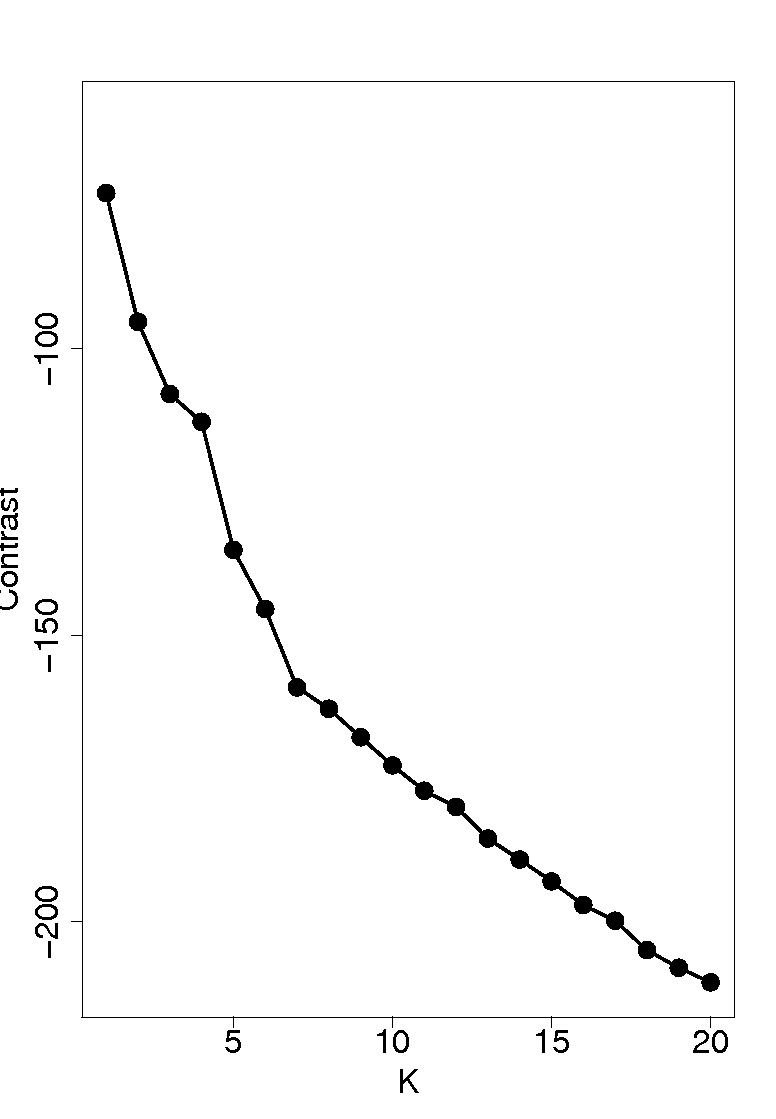
\includegraphics[width=.5\textwidth, height=.7\textheight]{../Figures/Bt474-J} 
    	\onslide<3>
    	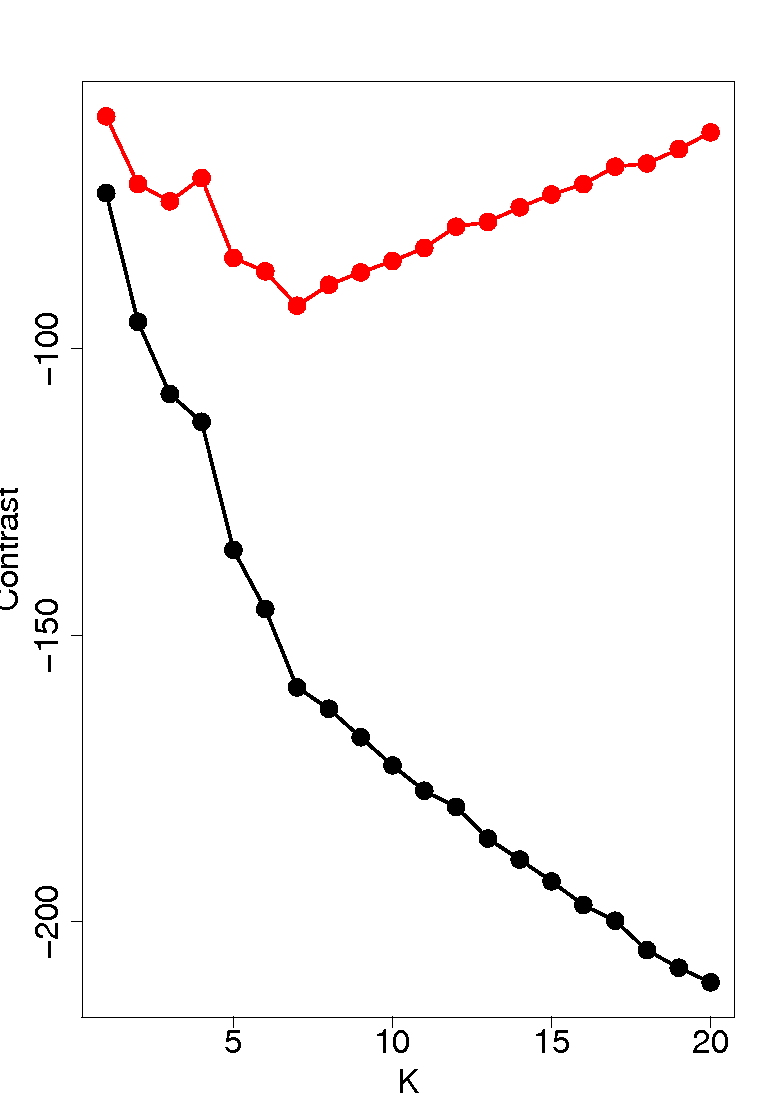
\includegraphics[width=.5\textwidth, height=.7\textheight]{../Figures/Bt474-JP} 
    	\onslide<4->
    	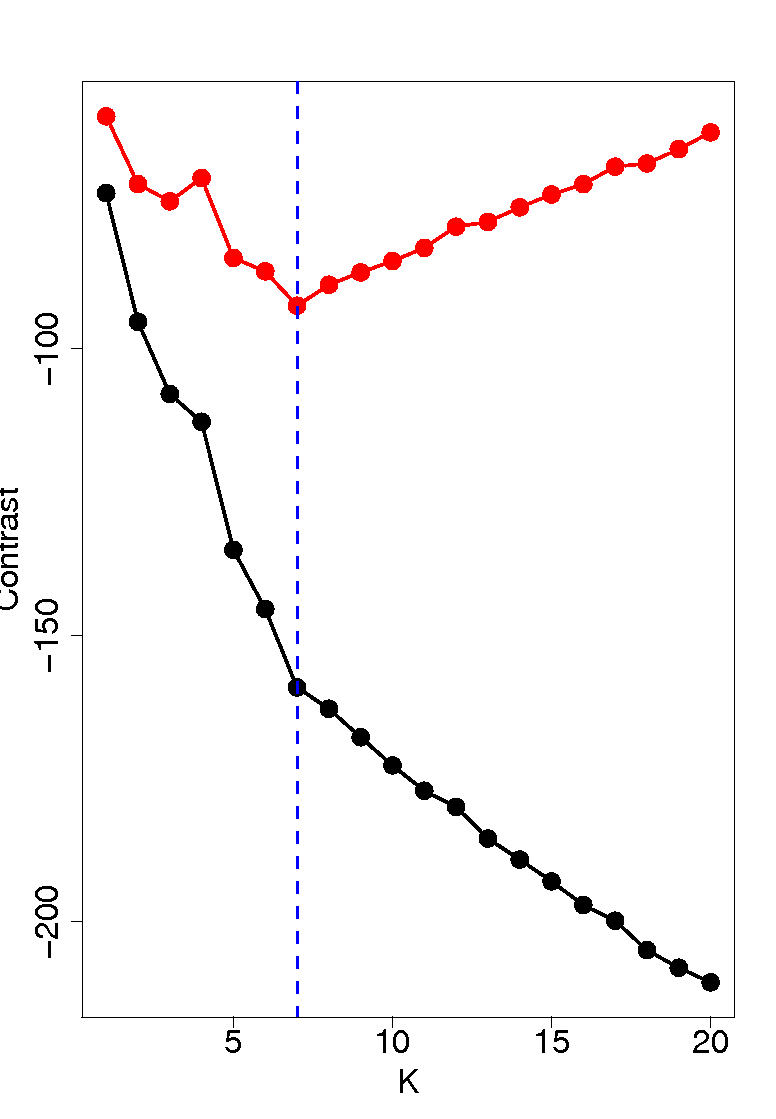
\includegraphics[width=.5\textwidth, height=.7\textheight]{../Figures/Bt474-JPM} 
    	\end{overprint}
    \end{tabular} 
  \end{tabular} 

  \onslide+<5>{ 
    \vspace{-.5cm} An abundant literature has been developed
    (\refer{Leb05}, \refer{Lav05}, \refer{ZhS07}, ...) to insure that
    $\Pr\{\widehat{K} = K\} \rightarrow 1$ when $n \rightarrow \infty$
    or to approximate $p(K | \Ybf)$.  }
  
}

%====================================================================
\frame{\frametitle{Penalization}

  Penalty 'calibration' requires theoretical developments, each dedicated to a specific model

  \begin{itemize}
    \item Gaussian homoscedastic (\refer{Leb05}) :  
    $$
    pen(K) = \frac{K}{n} \left(\log\dfrac{n}{K} +2.5\right) 
    $$ 
    \item Negative Binomial (\refer{ClL13}): 
    $$
    pen(K) = \frac{K}n \left(1+4\sqrt{1.1+\log\frac{n}{K}}\right)^2 
    $$
  \end{itemize}
}

%====================================================================
\subsection*{In practice}

%====================================================================
\frame{\frametitle{Illustration on RNA-seq}

  \paragraph{Detection of transcribed regions using RNA-seq.} Yeast chromosome 1 \refer{ClL13}\\

  \bigskip
  \begin{overprint}
   \onslide<1> 
    \text{Poisson model: 106 segments} 
    $$
    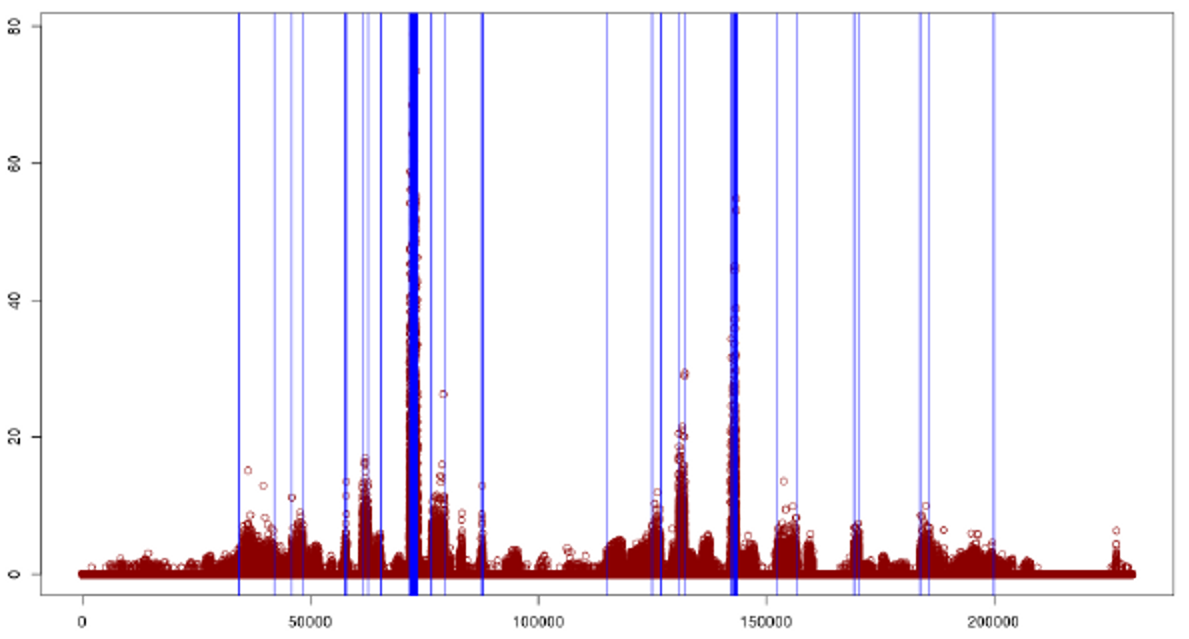
\includegraphics[width = .8\textwidth]{../Figures/ClL13-Fig2}
    $$
   \onslide<2> 
    \text{Negative binomial model: 103 segments} 
    $$
    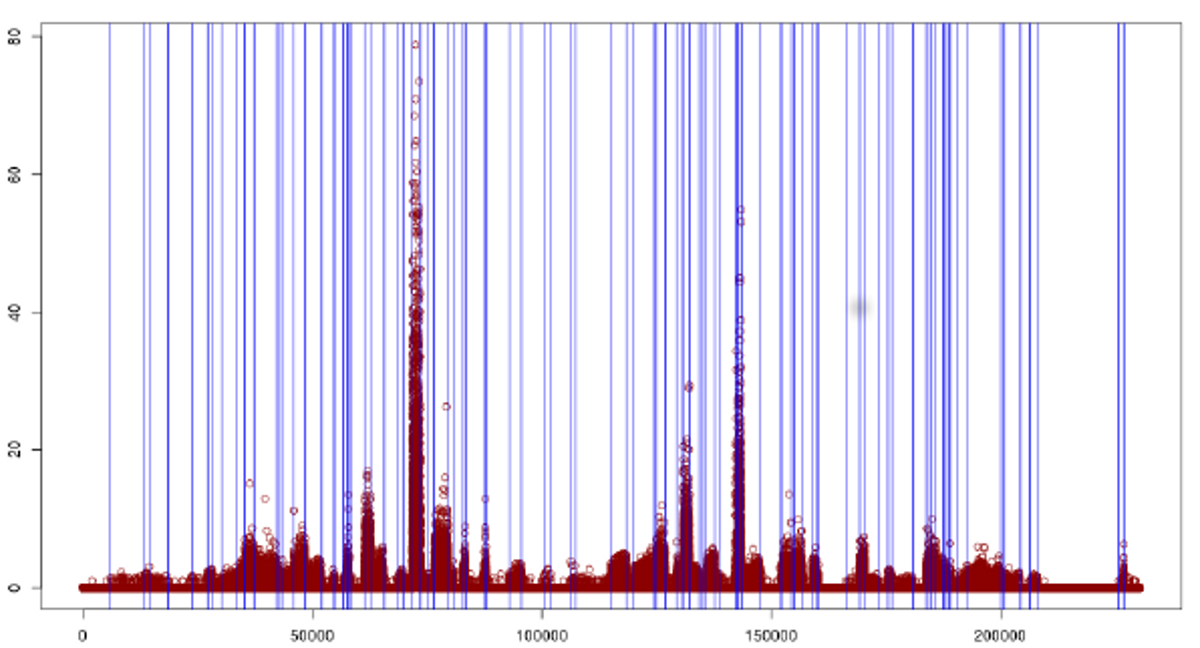
\includegraphics[width = .8\textwidth]{../Figures/ClL13-Fig3}
    $$
  \end{overprint}
}

%====================================================================
%====================================================================
\section[Reminder on Bayesian inference]{A (brief) reminder on Bayesian inference}
\frame{\frametitle{A (brief) reminder on Bayesian inference}}
%====================================================================

%====================================================================
\frame{\frametitle{A (brief) reminder on Bayesian inference}

  \paragraph{General statistical approach.}
  \begin{itemize}
   \item Observed data $Y = $ realization of a random phenomenon governed by some unknown parameter $\theta$.
   \item Model = description on how the distribution of $Y$ depends on $\theta$: $Y \sim p_\theta$.
   \item Statistical inference = being able to say something on $\theta$ based on $Y$.
  \end{itemize}

  \pause \bigskip
  \paragraph{Bayesian setting.}
  \begin{itemize}
  \item $\theta$ itself is random with '\emphase{prior}' (= marginal) distribution $p(\theta)$.
  \item The model gives the conditional distribution (= \emphase{likelihood}) of the data $Y$ given the parameter: $p(Y|\theta)$.
  \item Statistical inference = give the '\emphase{posterior}' (= conditional) distribution of the parameter given the observations $p(\theta|Y)$.
  \end{itemize}
  }

%====================================================================
\frame{\frametitle{Binomial experiment: classical inference}

  \paragraph{Problem.}
  Consider a treatment $A$ and let $\pi$ denote the probability for a patient to be cured when receiving $A$.
  
  \bigskip \pause
  \paragraph{Model.}
  Consider independent $n$ patients treated with $A$ and denote $Y$ the number of cured patients (= successes). We have
  $$
  Y \sim \Bcal(n, \pi)
  \pause \quad \Rightarrow \quad
  p_\pi(y) = \binom{n}{y} \pi^y (1-\pi)^{n-y}
  $$
  
  \bigskip \pause
  \paragraph{Classical (= frequentist) inference.} An estimate of $\pi$ is given by 
  $$
  \widehat{\pi} = Y/n.
  $$
  Its standard deviation is $\pi(1-\pi)/n$ and a confidence interval can be computed as well.

}

%====================================================================
\frame{\frametitle{Binomial experiment: Bayesian inference}

 \begin{tabular}{cc}
  \begin{tabular}{p{.45\textwidth}}
    \onslide+<1->{\paragraph{Prior.} Define a prior distribution $p(\pi)$ (e.g. you know nothing about it). \\ ~\\}
    \onslide+<2->{\paragraph{Data.} Observe the results of the experiment (e.g. $y = 4$ / $n=20$). \\ ~\\} 
  \onslide+<3->{\paragraph{Posterior.} Calculate the posterior of $\pi: p(\pi|Y=y)$. \\} 
  \end{tabular}
  &
  \begin{tabular}{p{.5\textwidth}}
    \hspace{-.05\textwidth}
    \begin{overprint}
    \onslide<1>\includegraphics[width=.45\textwidth]{../Figures/Fig-BetaBinomial-a1-b1-y4-n20-prior.pdf}
    \onslide<2>\includegraphics[width=.45\textwidth]{../Figures/Fig-BetaBinomial-a1-b1-y4-n20-prior-data.pdf}
    \onslide<3->\includegraphics[width=.45\textwidth]{../Figures/Fig-BetaBinomial-a1-b1-y4-n20-all.pdf}
    \end{overprint}
  \end{tabular}
 \end{tabular}

  
  \onslide+<4>{\paragraph{Inference.} An estimate is given by the posterior mode (i.e. the mode of $p(\theta|Y)$), a credibility interval can be computed as well.}
}

%====================================================================
\frame{\frametitle{Binomial experiment: Influence of the prior}

 \begin{tabular}{cc}
  \begin{tabular}{p{.45\textwidth}}
    \onslide+<1->{\paragraph{Flat prior:} You know nothing about it. \\ ~\\}
    \onslide+<2->{\paragraph{Jeffrey's prior.}\\ ~\\}
    \onslide+<3->{\paragraph{Expert prior:} Based on some previous knowledge. \\ ~\\}
  \end{tabular}
  &
  \begin{tabular}{p{.5\textwidth}}
    \hspace{-.05\textwidth}
    \begin{overprint}
    \onslide<1>\includegraphics[width=.45\textwidth]{../Figures/Fig-BetaBinomial-a1-b1-y4-n20-all.pdf}
    \onslide<2>\includegraphics[width=.45\textwidth]{../Figures/Fig-BetaBinomial-a05-b05-y4-n20-all.pdf}
    \onslide<3>\includegraphics[width=.45\textwidth]{../Figures/Fig-BetaBinomial-a8-b3-y4-n20-all.pdf}
    \onslide<4>\includegraphics[width=.45\textwidth]{../Figures/Fig-BetaBinomial-y4-n20-comp-prior.pdf}
    \end{overprint}
  \end{tabular}
 \end{tabular}

}

%====================================================================
\frame{\frametitle{Computation of the posterior}

  \paragraph{Aim:} We want to compute $p(\theta|Y)$ using Bayes' formula:
  $$
  p(\theta|Y) = \frac{p(\theta, Y)}{p(Y)} = \frac{p(\theta) p(Y|\theta)}{\int p(Y|\theta) p(\theta) \dd \theta} 
  $$
  where
  \begin{itemize}
   \item $p(\theta)$ is the known prior,
   \item $p(Y|theta)$ is the likelihood of the data (hopefully computable),
   \item $\int p(Y|\theta) p(\theta) \dd \theta$ is the normalizing constant that need to be computed.
  \end{itemize}

}

%====================================================================
\frame{\frametitle{Beta-Binomial case $(\theta = \pi$) (1/2)}

  Taking $\pi \sim \Beta(a, b)$:
  $$
  p(\pi) = \frac1{\text{B}(a, b)} \pi^{a-1} (1-\pi)^{b-1} = \frac{\Gamma(a+b)}{\Gamma(a) \Gamma(b)} \pi^{a-1} (1-\pi)^{b-1},
  $$ \pause
  because
  $$
  p(Y=y|\pi) = \binom{n}{y} \pi^y (1-\pi)^{n-y} %= \frac{\Gamma(n+1)}{\Gamma(y+1) \Gamma(n-y+1)} \pi^y (1-\pi)^{n-y}
  $$ \pause
  we get the normalizing constant
  $$
  \int p(Y=y|\pi) p(\pi) \dd \pi 
  = \binom{n}{y}  \frac{\Gamma(a+b)}{\Gamma(a) \Gamma(b)} \frac{\Gamma(y+a)  \Gamma(n-y+b)}{\Gamma(n+a+b)}.
%   = \frac{\Gamma(a+b)\Gamma(n+1)}{\Gamma(y+1) \Gamma(n-y+1) \Gamma(a) \Gamma(b)} \frac{\Gamma(y+a)  \Gamma(n-y+b)}{\Gamma(n+a+b)}.
  $$
%   \begin{eqnarray*}
%    & = & \int \frac{\Gamma(a+b)\Gamma(n+1)}{\Gamma(y+1) \Gamma(n-y+1) \Gamma(a) \Gamma(b)} \pi^{a-1} (1-\pi)^{b-1} \pi^y (1-\pi)^{n-y} \dd \pi \\
%    & = & \frac{\Gamma(a+b)\Gamma(n+1)}{\Gamma(y+1) \Gamma(n-y+1) \Gamma(a) \Gamma(b)} \int \pi^{y+a-1} (1-\pi)^{n-y+b-1} \dd \pi \\
%    \int p(y|\pi) p(\pi) \dd \pi & = & \frac{\Gamma(a+b)\Gamma(n+1)}{\Gamma(y+1) \Gamma(n-y+1) \Gamma(a) \Gamma(b)} \frac{\Gamma(y+a)  \Gamma(n-y+b)}{\Gamma(n+a+b)}
%   \end{eqnarray*}
}

%====================================================================
\frame{\frametitle{Beta-Binomial case $(\theta = \pi$) (2/2)}

  As a result, we get
  \begin{eqnarray*}
   p(\pi|Y=y) & = & p(\pi) p(y|\pi) \left/ \int p(\pi) p(y|\pi) \dd \pi \right. \\
   & = & \frac{\Gamma(n+a+b)}{\Gamma(y+a)\Gamma(n-y+b)} \pi^{y+a-1} (1-\pi)^{n-y+b-1},
  \end{eqnarray*} 
  \pause
  which we recognize as a Beta distribution $\Beta(a+y, b+n-y)$:
  $$
  (\pi | Y=y) \sim \Beta(\widetilde{a}, \widetilde{b})
  $$
  where
  $$
  \widetilde{a} = a+y, \qquad \widetilde{b} = b+n-y.
  $$
  
  \bigskip \pause
  Such a nice property is called \emphase{conjugacy}.
}

%====================================================================
\frame{\frametitle{Exercise: Gaussian linear regression}

  Take 
  $$
  \beta \sim \Ncal(b, \Sigma)
  $$
  and, for a design $n \times p$ matrix $X$,
  $$
  Y \sim \Ncal_n(X \beta, \sigma^2)
  $$
  prove that
  $$
  \beta|Y \sim \Ncal\left(\widetilde{b}, \widetilde{\Sigma}\right)
  $$
  where
  $$
  \widetilde{b} = \widetilde{\Sigma} \left(\Sigma^{-1} b + X'Y\right),
  \qquad
  \widetilde{\Sigma} = \left(\Sigma^{-1} + X'X\right)^{-1}.
  $$
  
  \bigskip \bigskip \pause
  \paragraph{Hint.} Have a look at \refer{Ban08} and see also how to deal with $\sigma^2$.
}

%====================================================================
\frame{\frametitle{What should we learn from all this?} 

  \paragraph{Bayesian inference}
  \begin{enumerate}
   \item considers the parameter $\theta$ as random and focus the inference on its posterior distribution;
   \item strongly relies on the calculation of possibly complex integrals or sums.
  \end{enumerate}

  \bigskip \pause
  \paragraph{Three main approaches} when the calculation of the posterior  becomes complex:
  \begin{itemize} \pause
   \item Sampling: design a (stochastic) algorithm to sample in $p(\theta|Y)$ \\
   \ra MCMC methods; \pause
   \item Approximation: derive an approximate distribution $q(\theta)  \simeq p(\theta|Y)$ \\
   \ra variational approaches; \pause
   \item Strong headed: still try to compute it exactly.
  \end{itemize}


}

%====================================================================
%====================================================================
\section{Exact posterior distributions in change point models}
%====================================================================
\frame{\frametitle{Exact posterior distribution in change point models \refer{RLR11}}}

%====================================================================
\frame{\frametitle{Bayesian framework for one series} 

  \paragraph{Number of segments:}
  $$
  K \sim p(K)
  $$ 

  \medskip
  \paragraph{Segmentation:}
  $$
  m = (\tau_k)_k \sim p(m|K)
  $$
  \ra Change points: $1 = \tau_0 < \dots < \tau_{K-1} < \tau_K = n +1$ \\
  \ra Segment:  $r \in m: r = \llbracket \tau_{k-1}, \tau_k \llbracket$

  \bigskip
  \paragraph{Parameters:}
  $$
  \theta = (\theta_r)_{r \in m} \sim p(\theta |m)
  $$

  \medskip
  \paragraph{Data:}
  $$
  Y = (Y_t)_{1 \leq t \leq n} \sim p(Y | \theta, m)
  $$


%   \begin{tabular}{lll}
%     Number of segments: & $K$ & $p(K)$ \\
%     ~ \\
%     Segmentation: & $m = (\tau_k)_k$ & $p(m|K)$ \\
%     (change points: & $0 < \tau_1 < \dots < \tau_{K-1} < n$) & \\
%     ~ \\
%     Segmentation space: & $\Mcal_K = \Mcal_K(\llbracket 1, n+1 \llbracket)$ & \\
%     ~ \\
%     Segment: & $r = \llbracket \tau_{k-1}, \tau_k \llbracket$ & \\
%     ~ \\
%     Parameters: & $\theta = (\theta_r)_{r \in m}$ & $p(\theta |m)$ \\
%     (segments: & $r = \llbracket \tau_{k-1}, \tau_k \llbracket$) & \\
% 
%     ~ \\
%     Data: & $Y = (Y_t)_{1 \leq t \leq n}$ & $p(Y | \theta, m)$ \\
%   \end{tabular}

  }

%====================================================================
\frame{\frametitle{Standard change point model} 

  \begin{tabular}{cc}
    \hspace{-.5cm}
    \begin{tabular}{p{.5\textwidth}}
      \onslide+<1->{\paragraph{Hierarchical model.} 
        \begin{itemize}
        \item \onslide+<2->{$K \sim p(K)$ \\~}
        \item \onslide+<3->{$m = (\tau_k)_k \sim p(m|K)$\\~}
        \item \onslide+<4->{$\theta = (\theta_r)_{r \in m} \sim p(\theta |m)$\\~}
        \item \onslide+<5->{$Y = (Y_t)_{1 \leq t \leq n} \sim p(Y | \theta, m)$}
        \end{itemize}}
    \end{tabular}
    & 
    \hspace{-1cm}
    \begin{tabular}{c}
%       \onslide+<2->{
%         \hspace{-6cm}
%         \onslide+<3->{if $t \in \textcolor{blue}{r_k}$,} \quad $Y_t$
%         \onslide+<5->{$\sim
%           \Fcal($}\onslide+<4->{$\textcolor{red}{\theta_k}$}\onslide+<5->{$)$}
%         \\}
      \begin{overprint}
        \onslide<2>
        \includegraphics[width=.5\textwidth]{../Figures/FigSeg-Budapest-1} 
        \onslide<3>
        \includegraphics[width=.5\textwidth]{../Figures/FigSeg-Budapest-2} 
        \onslide<4>
        \includegraphics[width=.5\textwidth]{../Figures/FigSeg-Budapest-3} 
        \onslide<5>
        \includegraphics[width=.5\textwidth]{../Figures/FigSeg-Budapest-4} 
        \onslide<6>
        \includegraphics[width=.5\textwidth]{../Figures/FigSeg-Budapest-0} 
%         \onslide<7->
%         \paragraph{Graphical model:} \\
%         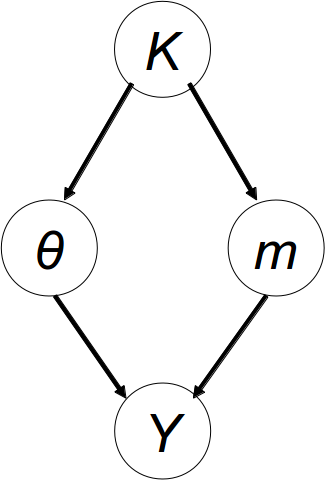
\includegraphics[width=.2\textwidth]{../Figures/EBS-GraphModel} \\
      \end{overprint}
    \end{tabular}
  \end{tabular}

  \onslide+<6->{
  $$
  \text{\emphase{Aim:} \qquad } p(K, m, \theta | Y)
  $$
  } 
}

%====================================================================
\frame{\frametitle{Posterior distribution} 

  \begin{tabular}{cc}
    \begin{tabular}{p{.65\textwidth}}
	 \begin{eqnarray*}
	 p(K, m, \theta | Y) 
	 & = & \frac{p(K, m, \theta, Y)}{p(K, m, \theta | Y)} \\
	 & = & \frac{p(K) p(m|K) p(\theta|K) p(Y|m, \theta)}{p(Y)} \\ 
	 \end{eqnarray*}
    \end{tabular}
    &
    \begin{tabular}{p{.3\textwidth}}
	 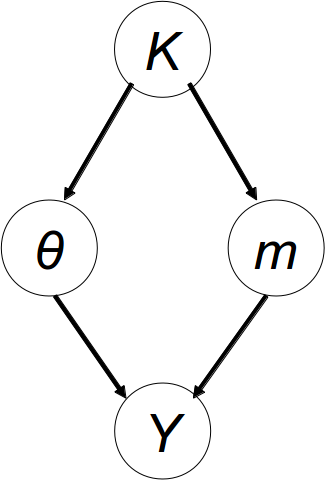
\includegraphics[width=.2\textwidth]{../Figures/EBS-GraphModel}
    \end{tabular}
  \end{tabular}
  
  \pause \bigskip
  The calculation sums and integral is required
  \begin{eqnarray*}
  p(Y) 
  & = & \sum_K \sum_{m \in \Mcal_K} \int p(K) p(m|K) p(\theta|K) p(Y|m, \theta) \dd \theta \\
  & = & \sum_K p(K) \sum_{m \in \Mcal_K} p(m|K) \int p(\theta|K) p(Y|m, \theta) \dd \theta \\
  \end{eqnarray*}
  
}

%====================================================================
\frame{\frametitle{Some distributions of interest} 

  %Infer several quantities based on the observed series $Y$.
  \begin{itemize}
   \item Number of change points: 
   $$
   p(K | Y)
   $$
   \item Change point location: 
   $$
   P\{\tau_k = t | Y\} \quad \text{or} \quad P\{\tau_k = t | Y, K\}
   $$
   \item Existence of a change point: 
   $$
   P\{\exists k: \tau_k = t | Y\}
   $$
   \item Reliability of the 'best' segmentation: 
   $$
   p(\widehat{m} | Y) \quad \text{or} \quad  p(\widehat{m} | Y, K)
   $$
   \item Mean of the parameter at a given location: 
   $$
   \Esp(\theta_t | Y)
   $$
  \end{itemize}
  }
  
  
%====================================================================
\frame{\frametitle{Factorability assumptions} 

  %We require that prior distribution satisfy the following.
  
   \begin{itemize}
   \item Segmentation:
   $$
   p(m|K) = \prod_{r \in m} f(r) 
   $$
   \ra $p(m|K) = 1 \left/ |\Mcal_K| \right.$ or $p(m|K) \propto \prod_{r \in m} n_r$ \\ ~
  \item Parameter:
  $$
  p(\theta|m) = \prod_{r \in m} f(\theta_r)
  $$
  \ra independent parameters in each segment (\emphase{no homoscedasticity}) \\ ~
  \item Data:
  $$
  p(Y | m, \theta) = \prod_{r \in m} f(Y^r, \theta_r) 
  $$
  \ra data are independent from one segment to another %(but not necessarily within each segment)
   \end{itemize}
}

%====================================================================
\frame{\frametitle{Need for integrals and sums} 

  \paragraph{Model selection:} $p(K | Y) \propto p(Y | K) p(K)$
  $$
  p(Y|K) = \sum_{m \in \Mcal_K} \prod_{r\in m} \int p(Y^r|\theta_r) p(\theta_r)
  \dd \theta_r = \sum_{m \in \Mcal_K} \prod_{r\in m} p(Y^r)
  $$
  $p(Y^r)$ has a close-form when using conjugate priors

  \bigskip \bigskip 
  \paragraph{Localisation of the $k$-th breakpoint:}
  \begin{eqnarray*}
    P\{\tau_k = t | K, Y\} & \propto & \left(\sum_{m \in \Mcal_k(1, t)} \prod_{r
    \in m} p(Y^r)\right) \left(\sum_{m \in \Mcal_{K-k}(t+1, n)} \prod_{r
    \in m} p(Y^r)\right)
  \end{eqnarray*}
  
  \bigskip 
  \ra Need to sum up over the whole segmentation space $\Mcal_K$.
  }

%====================================================================
\frame{ \frametitle{Computing sums of products}

To compute
  $$
  \sum_{m \in \Mcal_K(1, t)} \prod_{r \in m} f(r),
  $$
  define the upper triangular $(n+1) \times (n+1)$ matrix $A$:
  $$
  A_{ij} = f(\llbracket i, j \llbracket ), \qquad 1 \leq i < j \leq n+1
  $$
  then
  $$
  \sum_{m \in \Mcal_K(1,t)} \prod_{r \in m} f(r) = [A^k]_{1,t+1}
  $$
  \ra all terms ($1 \leq k \leq K$, $1 \leq t \leq n+1$) are computed in {$O(K n^2)$}.  
  
  \bigskip \bigskip
  \paragraph{NB:} Similar to the shortest path dynamic programing algorithm, replacing {'max'} with {'sum'} and {'sum'} with {'product'}
  }

%====================================================================
\frame{ \frametitle{A CGH profile: $K = 3, 4$}
 
 \vspace{-.25cm}
  \begin{tabular}{lll}
    \hspace{-0.5cm}
    \begin{tabular}{p{0.25\textwidth}} 
    %Optimal segmentation
    $\widehat{m}_K =$ \\
    $\arg\max_m p(m | Y ,K)$ 
    \end{tabular}
    &
    \hspace{-0.5cm}
    \begin{tabular}{c}
      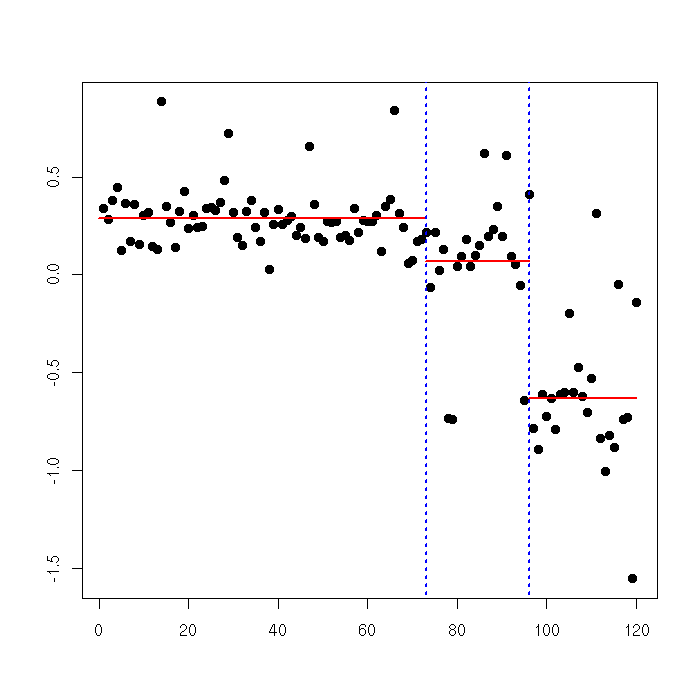
\includegraphics[width=0.3\textwidth, height=0.3\textheight,
      clip=]{../Figures/CopyNumberChr10_BIC}   
    \end{tabular}
    &
    \hspace{-0.5cm}
    \begin{tabular}{c}
      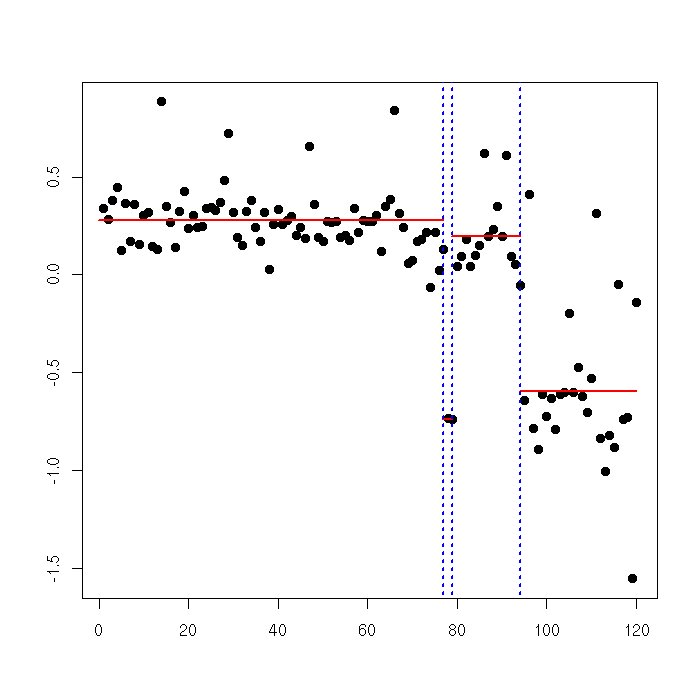
\includegraphics[width=0.3\textwidth, height=0.3\textheight,
      clip=]{../Figures/CopyNumberChr10_ICL}  
    \end{tabular}\\ 
    \hspace{-0.5cm}
    \begin{tabular}{p{0.25\textwidth}} 
    %Breakpoint position 
    $P\{\tau_K = t | Y, K\}$
    \end{tabular}
    &
    \hspace{-0.5cm}
    \begin{tabular}{c}
      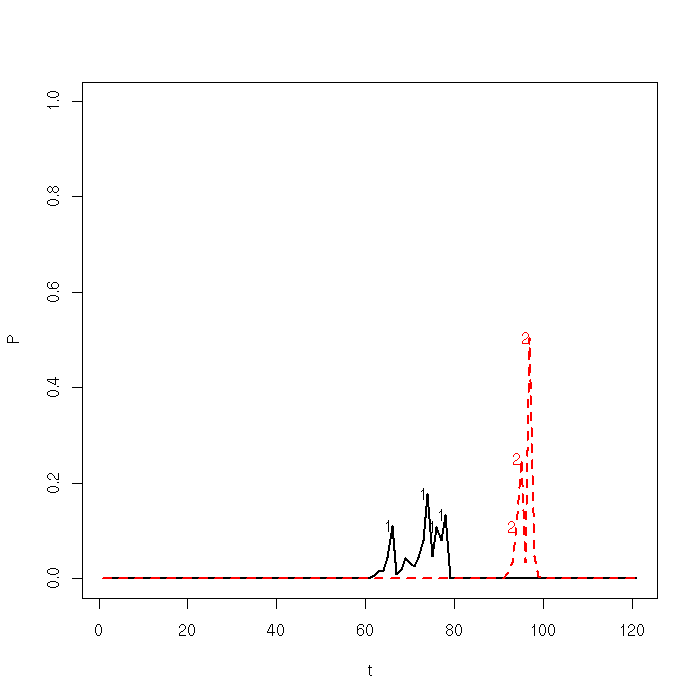
\includegraphics[width=0.3\textwidth, height=0.3\textheight,
      clip=]{../Figures/CopyNumberChr10_ProbaBIC}   
    \end{tabular}
    &
    \hspace{-0.5cm}
    \begin{tabular}{c}
      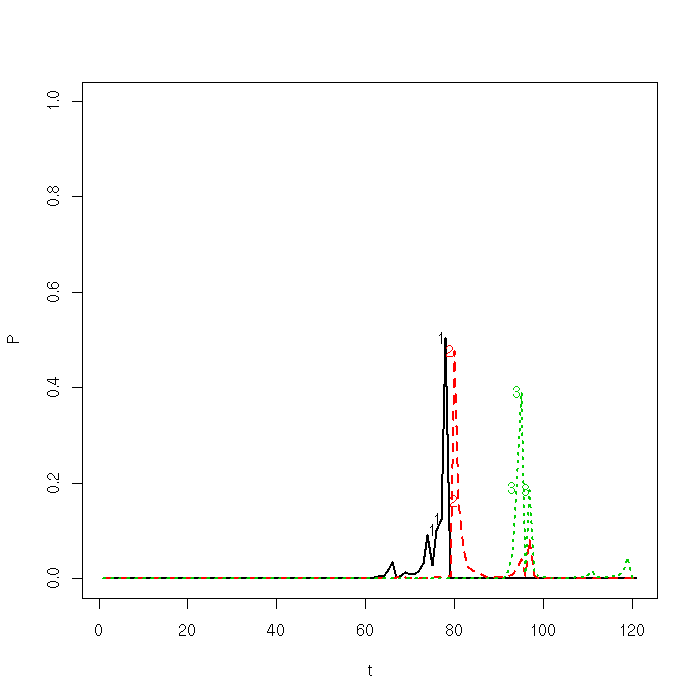
\includegraphics[width=0.3\textwidth, height=0.3\textheight,
      clip=]{../Figures/CopyNumberChr10_ProbaICL}  
    \end{tabular}\\ 
    \hspace{-0.5cm}
    \begin{tabular}{p{0.25\textwidth}} 
    %Segment probability 
    $P\{r \in m | Y, K\}$
    \end{tabular}
    &
    \hspace{-0.5cm}
    \begin{tabular}{c}
%      \vspace{-0cm}
      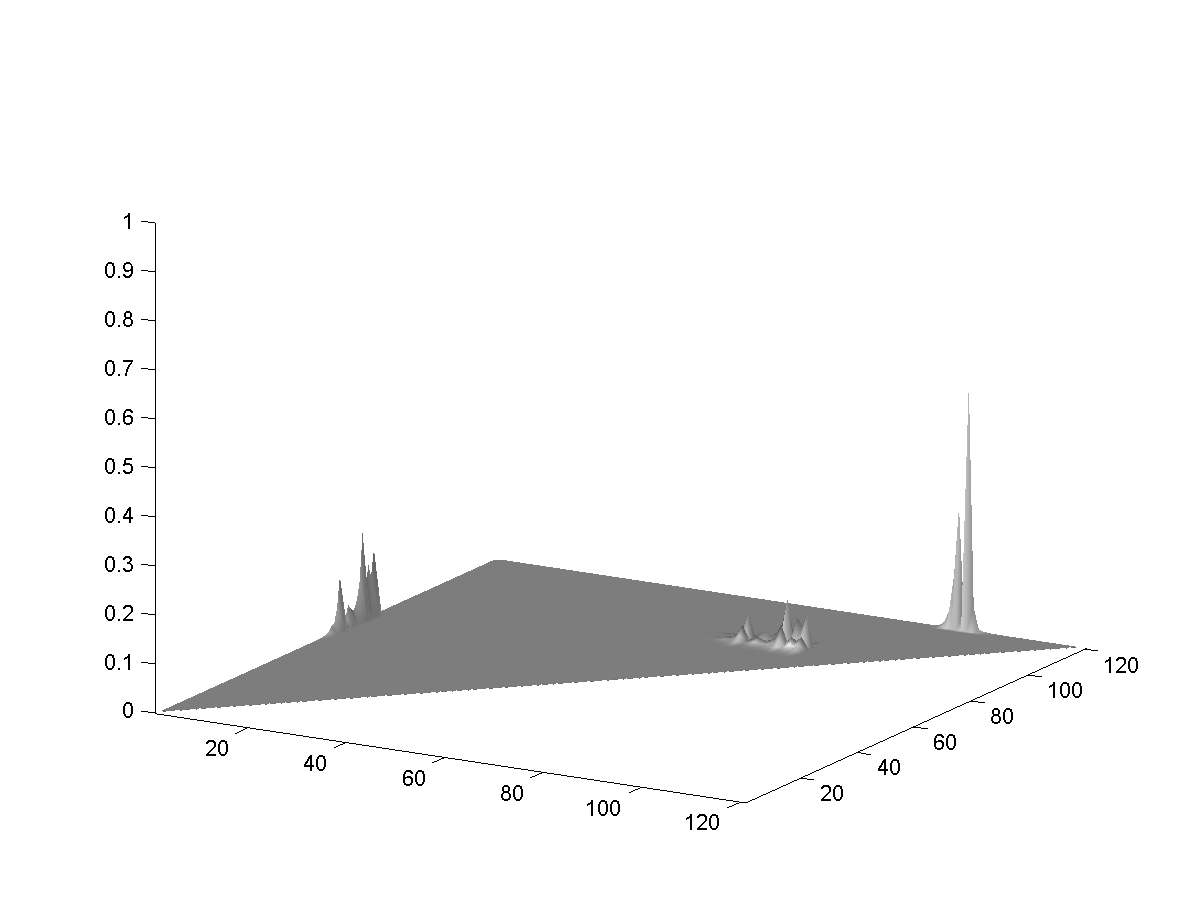
\includegraphics[width=0.32\textwidth, height=0.27\textheight,
      clip=]{../Figures/ProbSeg-BIC}     
    \end{tabular}
    &
%    \vspace{-.5cm}
    \begin{tabular}{c}
      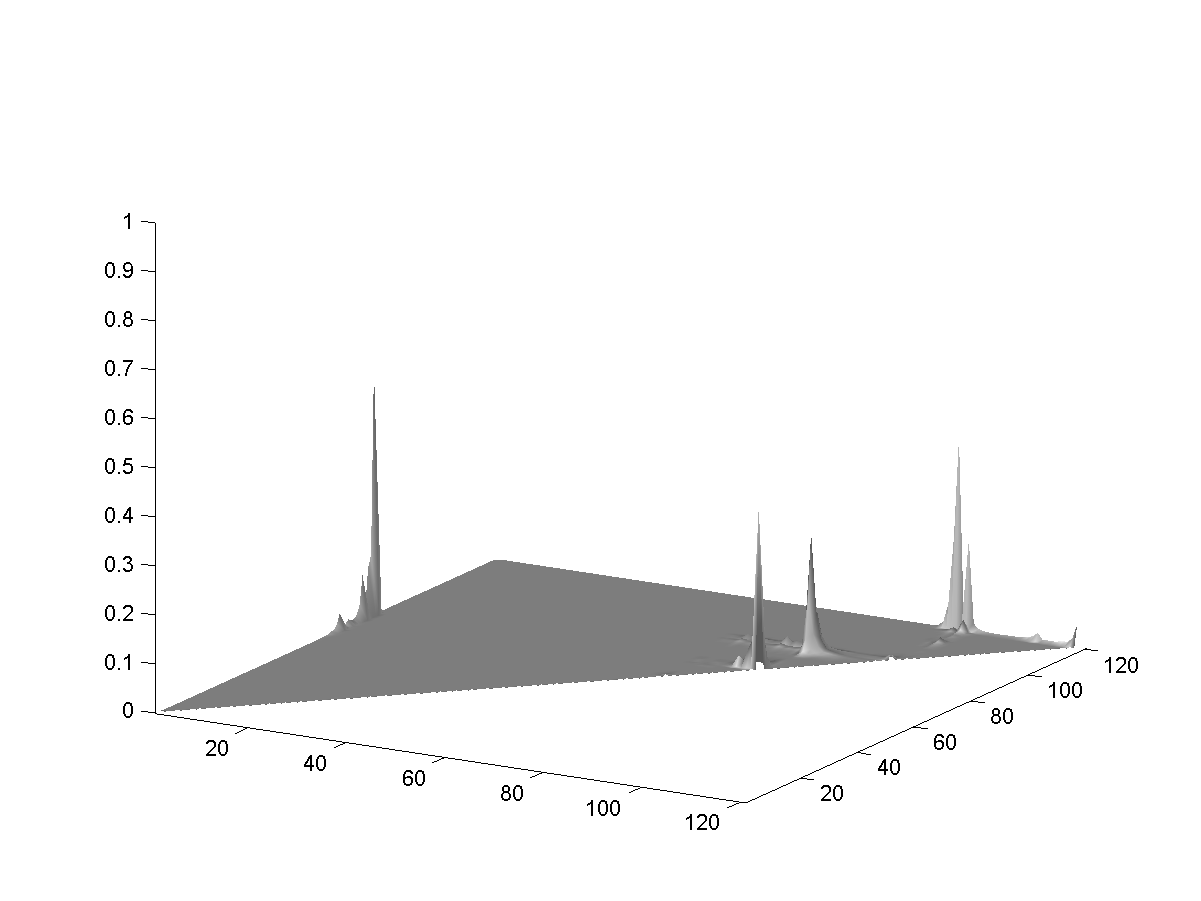
\includegraphics[width=0.32\textwidth, height=0.27\textheight,
      clip=]{../Figures/ProbSeg-ICL}   
    \end{tabular} 
  \end{tabular}
  }

%====================================================================
%====================================================================
\frame{ \frametitle{Model selection}

  \vspace{-.05\textwidth}
  \paragraph{Simulation:} Poisson signal alternating $\theta_0=1$ and $\theta_1$, $n = 100$. \\~

  \paragraph{Criterion} = \% of recovery of the true number of segments ($K = 5$). \\ 

  \begin{tabular}{p{.5\textwidth}p{.5\textwidth}}
    \hspace{-0.5cm}
    \begin{tabular}{p{.5\textwidth}}
	 \paragraph{Exact criteria} can be computed: \\ ~

	 $\textcolor{green}{BIC(K)} = \log p(Y, K)$ \\ ~

      $\textcolor{red}{BIC(m)} = \log p(Y, m)$ \\ ~
      
      $\textcolor{blue}{ICL(K)} = BIC(K) - H(K)$ \refer{BCG00} \\ ~\\
      $H(K) = $ entropy of $p(m | Y, K)$ 
    \end{tabular}
    &
    \hspace{-.05\textwidth}
    \vspace{-.3\textheight}
    \begin{tabular}{c}
% 	 \textcolor{green}{$BIC(K)$} \quad \textcolor{red}{$BIC(m)$} \quad
% 	 \textcolor{blue}{$ICL(K)$} \\
	 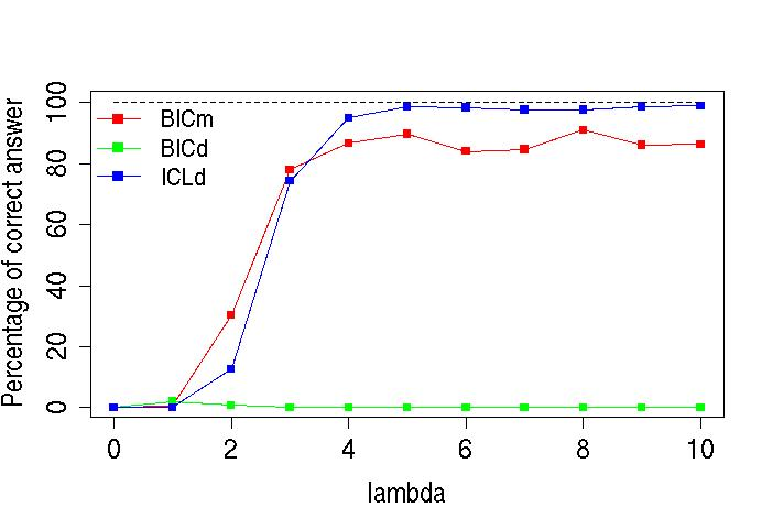
\includegraphics[width=.5\textwidth, height=.6\textheight]{../Figures/ICLvsBIC} \\ 
	 $\theta_1 - \theta_0, \quad \theta_0 = 1$
    \end{tabular}
  \end{tabular}
 }

%====================================================================
%====================================================================
\section{Comparing change point locations}
%====================================================================
\frame{\frametitle{Comparing change point locations  \refer{ClR14}}}

%====================================================================
\frame{\frametitle{RNA-seq data} 

  $$
  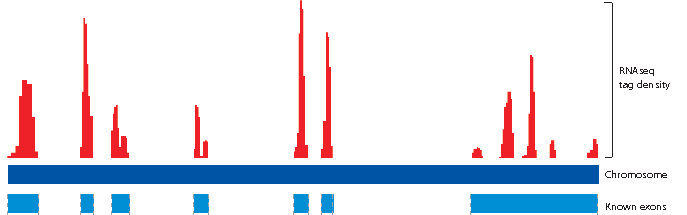
\includegraphics[width=.8\textwidth, height=.4\textheight]{../Figures/gb-2008-9-9-234-1}
  $$

  \bigskip \bigskip 
  \paragraph{New aim:} Determine if some boundaries of the transcribed regions may vary from one condition to another.
}

%====================================================================
\frame{\frametitle{Comparing transcript boundaries in yeast}

  \vspace{-.05\textheight}
  \begin{tabular}{p{.2\textwidth}p{.7\textwidth}}
    \begin{tabular}{p{.3\textwidth}}
	 One gene \\
	 \\
	 $\times$ \\
	 \\
	 Three growth \\
	 conditions: 
	 $A$, $B$, $C$
    \end{tabular}
    &
    \begin{tabular}{p{.7\textwidth}}
    \includegraphics[width=.7\textwidth]{../Figures/compyeastresult.pdf}
    \end{tabular}
  \end{tabular}
}

%====================================================================
\frame{\frametitle{Comparing 2 profiles}

  \paragraph{Model:} Two independent series $Y^1$ and $Y^2$

  \bigskip \bigskip
  \paragraph{Question:} Is there a shift between the two transcription starts?
  $$
  \Delta := \tau_1^1 - \tau_1^2 \overset{?}{=} 0
  $$
  
  \bigskip
  \paragraph{Posterior distribution of the shift:} 
  $$
  P\{\Delta=d|Y^1, Y^2, K^1, K^2\} 
  = \sum_t P\{\tau_ 1^1=t | Y^1, K^1\} P\{\tau_ 1^2 = t-d | Y^2, K^2\}
  $$
%   \begin{eqnarray*}
%   & & P\{\Delta=d|Y^1, Y^2, K^1, K^2\} \\
%   & & \qquad = \sum_t P\{\tau_ 1^1=t | Y^1, K^1\} P\{\tau_ 1^2 = t-d | Y^2, K^2\}   
%   \end{eqnarray*}
  
  \bigskip
  \paragraph{Application to RNAseq:}
  \begin{itemize}
  \item Consensus distribution: negative Binomial ${\mathcal NB}(\theta_r, \phi)$ 
  \item $\phi$ is first estimated using a robust moment-based estimator \refer{JKK92} (no common parameter allowed...)
  \item Exact posterior 95\% credibility intervals can then be derived
  \end{itemize}
 
}

%====================================================================
\frame{\frametitle{Back to the example}

  3 comparisons ($A/B$, $A/C$, $B/C$) $\times$ 4 change points:
  
\centerline{\includegraphics[width=.8\textwidth, height=.8\textheight]{../Figures/cred-yeast.pdf}}

}

%====================================================================
\frame{\frametitle{Comparing $I > 2$ profiles}

  \vspace{-0.5cm}
  \begin{tabular}{cc}
    \hspace{-0.5cm}
    \begin{tabular}{p{.6\textwidth}}
      \paragraph{Event of interest:} consider $I$ profiles
      $$
      E_0 = \{\tau_{k_1}^1 = \dots = \tau_{k_I}^I\}
      $$

      ~\\
      \paragraph{Aim: } evaluate the posterior
      $$
      P(E_0 | {\bf Y}, {\bf K})
      $$
%       can be computed exactly in ${\mathcal O}(In^2)$.
      
	 ~\\ ~\\
	 ${\bf Y} = (Y^1, \dots Y^I)$, 
	 ${\bf K} = (K^1, \dots K^I)$, ... 
    \end{tabular}
    &
    %\hspace{-.5cm}
    \begin{tabular}{c}
       \paragraph{Graphical model:} \\ ~\\
      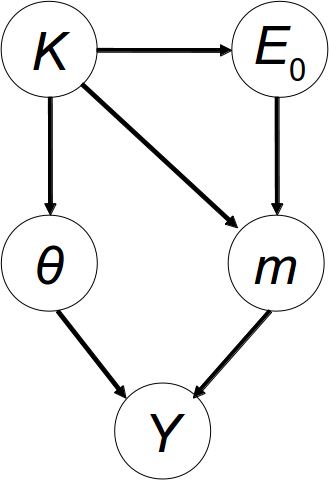
\includegraphics[width=.2\textwidth]{../Figures/EBS-GraphModel-E0}
    \end{tabular}
  \end{tabular}

  }

%====================================================================
\frame{\frametitle{Boundary shifts} 

  \paragraph{Efficient summation rules} only apply for independent series or given $E_0$ \\ 
  
  \begin{enumerate}
   \item Consider the surrogate model $Q$ where series are fully independent:
  \begin{eqnarray*} 
   Q(\Ybf, E_0 | \Kbf) & = & \sum_t \prod_\ell  \left[(A_\ell)^{k_\ell}\right]_{1, t} \left[(A_\ell)^{K_\ell-k_\ell}\right]_{t+1, n+1}\\
   Q(\Ybf | \Kbf) & = & \prod_\ell \left[(A_\ell)^{K_\ell}\right]_{1, n+1}
  \end{eqnarray*}
  \item Then, via probability change,
  \begin{eqnarray*} 
  & & P(E_0 | \Ybf, \Kbf) \\
  & = & \frac{p_0}{q_0} Q(\Ybf, E_0 | \Kbf) \left/
  \left[ \frac{p_0}{q_0} Q(\Ybf, E_0 | \Kbf) +  \frac{1 - p_0}{1 - q_0} Q(\Ybf, E_1 | \Kbf) \right] \right.
  \end{eqnarray*}
  where $E_1 = \overline{E}_0$, $p_0 = P(E_0 | \Kbf)$, $q_0 = Q(E_0 | \Kbf)$%, $Q(\Ybf, E_1 | \Kbf) = Q(\Ybf | \Kbf) - Q(\Ybf, E_0 | \Kbf)$
%   and $A_\ell$ stands for the matrix $A$ as defined in (\ref{eq:matrixA}), corresponding to series $\ell$.
  \end{enumerate}

  }

%====================================================================
\frame{\frametitle{Back to the example}

$$
\begin{array}{lccccc}
& \tau_1 & \tau_2 & \tau_3 & \tau_4 \\ 
\hline \\
P(E_0(A, B) | \Ybf, \Kbf) & 0.32 & 0.30 &0.99 & 10^{-5} \\ \\
P(E_0(A, C) | \Ybf, \Kbf) & 4 \; 10^{-4} & 0.99 &0.99 & 6 \; 10^{-3} \\ \\
P(E_0(B, C) | \Ybf, \Kbf) & 5 \; 10^{-2} & 0.60 & 0.99 & 0.99 \\ \\
P(E_0(A, B, C) | \Ybf, \Kbf) & 10^{-3} & 0.99  & 0.99 & 6 \; 10^{-3} \\ 
\end{array}
$$

\bigskip
\ra Differences at the UTR's end but not at internal exon boundaries.
}

%====================================================================
\frame{\frametitle{Various isoforms in yeast?} 

  \paragraph{$P(E_0|\Ybf, \Kbf)$} for yeast genes with 2 expressed exons
  $$
  \begin{tabular}{cc}
  \includegraphics[width=.4\textwidth]{../Figures/statall-all} 
  & 
  \includegraphics[width=.4\textwidth]{../Figures/statall2} 
  \\
   $p_0 = (.5, \;.5, \;.5, \;.5)$
   &
   $p_0 = (.9, \;.99, \;.99, \;.9)$
  \end{tabular}
  $$
}

%====================================================================
%====================================================================
\section*{Advertisement}
%====================================================================
\frame{\frametitle{Advertisement}

  R package available at {\tt cran.r-project.org}: \\~
  \begin{description}
   \item[EBS:] exact Bayesian segmentation, posterior probabilities of breakpoints, BIC and ICL criteria, comparison of change point location, (Gaussian, Poisson, negative binomial) \refer{ClR14}
  \end{description}
  + some related packages
  \begin{description}
   \item[CGHseg:] analysis of CGH and SNP  arrays for copy number variation analysis using segmentation models: one or several profiles, with/without covariates, with/without calling (Gaussian) \refer{PLH11} \\ ~
   \item[Segmentor3IsBack:] fast exact segmentation for various cost functions (Gaussian, Poisson, negative binomial) \refer{CKL14} \\ ~
  \end{description}
  }

%====================================================================
%====================================================================
\section*{Appendix}
%====================================================================

{\tiny
  \bibliography{/home/robin/Biblio/ARC,/home/robin/Biblio/AST,/home/robin/Biblio/SSB}
  %\bibliographystyle{/home/robin/LATEX/astats}
  \bibliographystyle{plain}
  }

%====================================================================
%====================================================================
\end{document}
%====================================================================
%====================================================================


\frame{\frametitle{}
  }

  \begin{tabular}{cc}
    \begin{tabular}{p{.5\textwidth}}
    \end{tabular}
    &
    \begin{tabular}{p{.5\textwidth}}
	 \begin{overprint}
	 \end{overprint}
    \end{tabular}
  \end{tabular}
